% Options for packages loaded elsewhere
\PassOptionsToPackage{unicode}{hyperref}
\PassOptionsToPackage{hyphens}{url}
\PassOptionsToPackage{dvipsnames,svgnames,x11names}{xcolor}
%
\documentclass[
  10pt,
]{article}
\usepackage{amsmath,amssymb}
\usepackage{iftex}
\ifPDFTeX
  \usepackage[T1]{fontenc}
  \usepackage[utf8]{inputenc}
  \usepackage{textcomp} % provide euro and other symbols
\else % if luatex or xetex
  \usepackage{unicode-math} % this also loads fontspec
  \defaultfontfeatures{Scale=MatchLowercase}
  \defaultfontfeatures[\rmfamily]{Ligatures=TeX,Scale=1}
\fi
\usepackage{lmodern}
\ifPDFTeX\else
  % xetex/luatex font selection
\fi
% Use upquote if available, for straight quotes in verbatim environments
\IfFileExists{upquote.sty}{\usepackage{upquote}}{}
\IfFileExists{microtype.sty}{% use microtype if available
  \usepackage[]{microtype}
  \UseMicrotypeSet[protrusion]{basicmath} % disable protrusion for tt fonts
}{}
\makeatletter
\@ifundefined{KOMAClassName}{% if non-KOMA class
  \IfFileExists{parskip.sty}{%
    \usepackage{parskip}
  }{% else
    \setlength{\parindent}{0pt}
    \setlength{\parskip}{6pt plus 2pt minus 1pt}}
}{% if KOMA class
  \KOMAoptions{parskip=half}}
\makeatother
\usepackage{xcolor}
\usepackage[margin=2.5cm]{geometry}
\usepackage{longtable,booktabs,array}
\usepackage{calc} % for calculating minipage widths
% Correct order of tables after \paragraph or \subparagraph
\usepackage{etoolbox}
\makeatletter
\patchcmd\longtable{\par}{\if@noskipsec\mbox{}\fi\par}{}{}
\makeatother
% Allow footnotes in longtable head/foot
\IfFileExists{footnotehyper.sty}{\usepackage{footnotehyper}}{\usepackage{footnote}}
\makesavenoteenv{longtable}
\usepackage{graphicx}
\makeatletter
\def\maxwidth{\ifdim\Gin@nat@width>\linewidth\linewidth\else\Gin@nat@width\fi}
\def\maxheight{\ifdim\Gin@nat@height>\textheight\textheight\else\Gin@nat@height\fi}
\makeatother
% Scale images if necessary, so that they will not overflow the page
% margins by default, and it is still possible to overwrite the defaults
% using explicit options in \includegraphics[width, height, ...]{}
\setkeys{Gin}{width=\maxwidth,height=\maxheight,keepaspectratio}
% Set default figure placement to htbp
\makeatletter
\def\fps@figure{htbp}
\makeatother
\setlength{\emergencystretch}{3em} % prevent overfull lines
\providecommand{\tightlist}{%
  \setlength{\itemsep}{0pt}\setlength{\parskip}{0pt}}
\setcounter{secnumdepth}{-\maxdimen} % remove section numbering
\ifLuaTeX
  \usepackage{selnolig}  % disable illegal ligatures
\fi
\IfFileExists{bookmark.sty}{\usepackage{bookmark}}{\usepackage{hyperref}}
\IfFileExists{xurl.sty}{\usepackage{xurl}}{} % add URL line breaks if available
\urlstyle{same}
\hypersetup{
  pdftitle={Silent Evidence Defects in the Wild: A Registered Replay of a Real Purchase-to-Pay Process},
  pdfauthor={Gaston Besanson, Universidad Torcuato Di Tella},
  colorlinks=true,
  linkcolor={Maroon},
  filecolor={Maroon},
  citecolor={Blue},
  urlcolor={Blue},
  pdfcreator={LaTeX via pandoc}}

\title{Silent Evidence Defects in the Wild: A Registered Replay of a
Real Purchase-to-Pay Process}
\author{Gaston Besanson, Universidad Torcuato Di Tella}
\date{}

\begin{document}
\maketitle

\hypertarget{abstract}{%
\subsection{Abstract}\label{abstract}}

Of the 155,534 analysed invoice clearings of a real purchase-to-pay
event log (Section 4 gives the registered exclusions), 17,748 (11.41\%,
clustered bootstrap 95\% interval {[}10.94\%, 11.92\%{]}) were made on
evidence that failed at least one of seven registered predicates,
carrying 19.41\% of the cleared value ({[}16.04\%, 23.09\%{]}). We
replay every analysed clearing of the BPI Challenge 2019 log through a
deterministic min() gate declared before the data were read, over the
evidence reconstructed from the log at clearing time. Clearings made on
evidence that failed on the goods receipt (absent or late, D1/D2) were
followed by a corrective event within 60 days at a rate of 5.64\%,
against 0.93\% for three-way clearings with every applicable predicate
passing (difference 0.0470, Holm-adjusted p = \(4.53 \times 10^{-4}\));
clearings made after a change of price or quantity since approval (D4
fail), at 1.91\% against 0.96\% for D4-pass clearings (difference
0.0094, Holm-adjusted p = \(3.48 \times 10^{-7}\)). On a registered
sample of lines with a failed predicate and of clean lines, two model
families shown the ERP view held 100.0\% and 99.6\% of the first and
53.0\% and 57.3\% of the second; on the sample lines the log lets us
classify, people held 33.0\% and 34.0\%, where a hold is an inferred
non-release within 60 days, not a recorded decision; the gate's verdict
holds the first and allows the second by construction. A line's status
at the decision point follows a reading of D5 (decision D-C-2 B) that
the author fixed after E3 and before any model call (Section 4). Paper
5's compiler, given the three declared losses of the registration, does
not reproduce the registered contract in any item category. The coverage
matrix states which defect classes this log cannot expose; the authority
defect class (D5) has zero incidence here. No causal claim is made.

\hypertarget{introduction}{%
\subsection{1 Introduction}\label{introduction}}

Earlier papers of this programme showed the mechanism of a silent
evidence defect, a decision taken on evidence that fails a
metadata-borne predicate, on constructed domains, and made no prevalence
claim: paper 4 (Besanson 2026a) and paper 5 (Besanson 2026b) are on
arXiv, and paper 6 is a public repository (Besanson 2026c). We found no
record that identifies papers 1 to 3, and do not cite them. This paper
is the number, on one real process.

The unit is an invoice clearing in the BPI Challenge 2019
purchase-to-pay log. For each of the 155,534 analysed clearings (the
exclusion table of Section 4) we reconstruct the evidence recorded on
the purchase-order line at clearing time, evaluate the registered
predicates D1 to D7, record what the gate would have held, and read what
followed in the log. We report exposure in count and in anonymised EUR,
the corrective events that follow a failed predicate, the reach of the
gate, and, on a registered sample, what two model families decide on the
same ERP view beside the people in the log and the gate. Everything was
registered before the log was parsed beyond its published counts (tag
\texttt{prereg-p7-v1}) and amended once after the pilot (v1.1, tag
\texttt{prereg-p7-v1.1}), with four deviations under v1.1: two decided
after E2 and E3 and before E4, and two found in review (corrected
descriptions in the coverage matrix, and the E7 bootstrap replicates
with an empty group discarded); all are listed in Section 4.

What this paper claims is in the claim table of Appendix B. What it does
not claim is stated in the repository's claims file and repeated here
verbatim:

\begin{itemize}
\tightlist
\item
  No causal claim. Correctives are a proxy, observational, confounded by
  vendor, category and practice.
\item
  No loss figure. A corrected payment is not money gone; recovery is not
  in the log.
\item
  No claim that the gate stops anything. Held lines go somewhere the log
  does not show.
\item
  No claim about the company or any vendor. No company, subsidiary or
  vendor is named in any finding.
\item
  No agent acting on the live system and no agent with tools.
\item
  No readiness threshold.
\end{itemize}

``No claim about the company'' means that no company, subsidiary or
vendor is named or characterised; the measured process is the subject of
every finding.

\hypertarget{related-work}{%
\subsection{2 Related work}\label{related-work}}

This paper does not introduce conformance checking, the three-way match
or rework analysis. It replays each clearing as a gate decision over the
evidence reconstructed from the event log at clearing time, measures how
often that evidence was defective and what followed, and puts people,
models and the gate on the same lines. The defect classes are the
predicates of Section 3.

\textbf{Conformance and compliance checking.} Checking recorded
behaviour against a normative model or rule set is established (van der
Aalst 2016; Ly et al.~2015), and declarative constraints in the Declare
family take a process model as the conjunction of its constraints (Pesic
et al.~2007). The predicates D1 to D7 are compliance rules in this
sense, and taking the decision as their conjunction is Declare's.
Synthesising a sufficient contract from declared losses is paper 5 of
this programme (Besanson 2026b); the compiler used in Section 5.5 is
paper 5's. Detecting that one resource performed two activities that
must be separated is a standard compliance monitoring functionality (Ly
et al.~2015); predicate D5 is that check.

\textbf{The BPI Challenge 2019 reports.} The challenge posed the process
owner's compliance questions on this very log, including clearing before
goods receipt and the three-way match per item category (ICPM 2019). The
submitted reports measured basic violation rates and are prior art for
every basic rate reported here; among them Diba et al.~2019 quantify
receipt-before-clearing violations with their value, and Porter et
al.~2019 report compliance per item category both by number and by
value. Measuring compliance by count and by value is therefore not
claimed; what is claimed is the tabulation per clearing and per defect
class, with clustered intervals. The three-way match itself is a
textbook application control (PCAOB 2004); Section 5.5 asks whether
paper 5's compiler re-derives it from declared losses.

\textbf{Deviation and outcome.} Relating a deviation to a later outcome
in the same case is established: the extension of process mining to
outcomes associated with deviations (Peleg et al.~2008),
outcome-oriented predictive process monitoring (Teinemaa et al.~2019)
and deviance mining (Nguyen et al.~2016). On this log, Porter et
al.~2019 observe cancellations of invoice receipts long after clearing
as a case-study observation. Corrective events as rework signals are
established on this log too: Meyer zu Wickern et al.~2019 count change,
cancel and delete activities as rework, and Badakhshan et al.~2019 list
vendor debit memos among rework activities. The outcome proxy of Section
3 is a rework signal of this kind; H1 to H3 are registered
conditional-consequence studies of the deviation-to-outcome shape.

\textbf{Detectability.} That some deviations leave no trace in an event
log is established (Outmazgin and Soffer 2013). The registered per-class
coverage matrix of Section 6 is claimed; the principle is not.

\textbf{Deciders on the same cases.} Putting different deciders on the
same cases is established: a human reviewer, a model agent and learned
rules on the same accounts (Palma et al.~2026), language models against
audit baselines on the same ledgers (Kadir et al.~2025), and algorithms
against bank managers (Harding and Vasconcelos 2022). None of these uses
a deterministic contract declared before the data were read, or a human
arm read from a process event log; Section 5.4 does both, with one
qualification: the status of a line at the decision point follows a
reading of D5 (decision D-C-2 B) that the author fixed after E3 and
before any model call (Section 4).

\textbf{The BPI Challenge 2020 reports.} The 2020 challenge posed
questions on the approval chain of travel declarations (ICPM 2020b); two
reports received awards (ICPM 2020a; Pufahl et al.~2020; Kas et
al.~2020). They are prior art for the basic rates of the replication in
Section 5.7.

\hypertarget{formal-core}{%
\subsection{3 Formal core}\label{formal-core}}

\textbf{Lines, clearings and evidence.} A line is one case of the log:
one purchase document and item. A clearing is one
\texttt{Clear\ Invoice} event on a line at time t\_c.~The evidence at
t\_c is every event on the line with timestamp at most t\_c, excluding
the clearing itself, as the registration defines ``before t\_c''
(section 2 of \texttt{prereg-p7-v1}, unchanged in v1.1); events sharing
a timestamp count as available, and counts rather than event order
decide receipts, blocks and deletions, so the verdict does not depend on
the order of events with equal timestamps (a property test of the replay
engine).

\textbf{Category and contract.} The case flags select the contract, as
the data record states the rules:

\begin{longtable}[]{@{}
  >{\raggedright\arraybackslash}p{(\columnwidth - 6\tabcolsep) * \real{0.2500}}
  >{\raggedright\arraybackslash}p{(\columnwidth - 6\tabcolsep) * \real{0.2500}}
  >{\raggedright\arraybackslash}p{(\columnwidth - 6\tabcolsep) * \real{0.2500}}
  >{\raggedright\arraybackslash}p{(\columnwidth - 6\tabcolsep) * \real{0.2500}}@{}}
\toprule\noalign{}
\begin{minipage}[b]{\linewidth}\raggedright
category
\end{minipage} & \begin{minipage}[b]{\linewidth}\raggedright
GR-based invoice verification
\end{minipage} & \begin{minipage}[b]{\linewidth}\raggedright
goods receipt
\end{minipage} & \begin{minipage}[b]{\linewidth}\raggedright
contract
\end{minipage} \\
\midrule\noalign{}
\endhead
\bottomrule\noalign{}
\endlastfoot
three-way, invoice after receipt (\texttt{3-way}) & true & true & D1 to
D7 \\
three-way, invoice before receipt (\texttt{3-way}) & false & true & D1
to D7 \\
two-way (\texttt{2-way}) & false & false & D3 to D7 \\
consignment & any & any & excluded \\
\end{longtable}

\textbf{Predicates.} Each predicate takes the value pass, fail or
unknown; unknown means a required input is missing. Each predicate
checks one SARC-DQ dimension (the table). The contract as a whole is
checked with paper 5's own sufficiency function over this log's observed
states (E5, \texttt{results/e5/sufficiency.json}, Section 5.5): it is
sufficient for the three declared losses in the two-way category, and in
the two three-way categories for L1 and L3 but not for L2; it is minimal
in no category.

\begin{longtable}[]{@{}
  >{\raggedright\arraybackslash}p{(\columnwidth - 6\tabcolsep) * \real{0.2500}}
  >{\raggedright\arraybackslash}p{(\columnwidth - 6\tabcolsep) * \real{0.2500}}
  >{\raggedright\arraybackslash}p{(\columnwidth - 6\tabcolsep) * \real{0.2500}}
  >{\raggedright\arraybackslash}p{(\columnwidth - 6\tabcolsep) * \real{0.2500}}@{}}
\toprule\noalign{}
\begin{minipage}[b]{\linewidth}\raggedright
id
\end{minipage} & \begin{minipage}[b]{\linewidth}\raggedright
name
\end{minipage} & \begin{minipage}[b]{\linewidth}\raggedright
dimension
\end{minipage} & \begin{minipage}[b]{\linewidth}\raggedright
fails when, on the line before t\_c
\end{minipage} \\
\midrule\noalign{}
\endhead
\bottomrule\noalign{}
\endlastfoot
D1 & receipt present & presence & no uncancelled goods receipt (receipts
minus receipt cancellations at most zero) \\
D2 & receipt before clearing & freshness, order & no uncancelled receipt
precedes t\_c \\
D3 & invoice present & presence & no invoice receipt \\
D4 & unchanged since approval & validity & a price or quantity change
after the last approval-bearing event \\
D5 & distinct actors & authority & the actor of the clearing equals an
actor of the earliest creation (unknown if either is missing) \\
D6 & block respected & scope & payment blocks set minus blocks removed
greater than zero \\
D7 & not deleted & validity & deletions plus blocks minus reactivations
of the line greater than zero \\
\end{longtable}

At t\_c, D1 and D2 have the same truth value; they are kept apart
because they carry two dimensions. For reporting only, a D1/D2 failure
is assigned to a defect class by what the log records later: the stale
receipt (D2 class) if an uncancelled receipt is recorded after t\_c and
by the observation end, the absent receipt (D1 class) otherwise.

\textbf{Verdict.} The verdict is min() over the category's contract with
pass as one and fail or unknown as zero: the gate allows a clearing if
and only if every applicable predicate passes, and otherwise would have
held it. A clearing is defective if at least one applicable predicate
fails; one whose only non-pass value is unknown is held but not
defective, and is counted separately. ``Defect'' is used only for a
failed predicate.

\textbf{Human hold.} A line is held by people if a payment block is
recorded before its first clearing, or if no clearing is recorded within
W days of its first invoice receipt; a clearing before the first invoice
receipt counts as a release.

\textbf{Outcome proxy and lag bands.} O = 1 for a clearing if a
registered corrective activity (an invoice receipt or goods receipt
cancelled, a price or quantity changed, the line deleted, a vendor debit
memo, a subsequent invoice) is recorded on the line within W after t\_c;
W = 60 days, with W = 30 days as a descriptive sensitivity. For a D1/D2
failure, the lag from t\_c to the first uncancelled receipt falls in one
of the registered bands {[}0, 1{]}, (1, 7{]}, (7, 30{]} days, over 30
days, or never.

\textbf{Evidence set.} One record per analysed clearing carries the line
id (hashed in every export), category, t\_c, every predicate input and
value, the verdict, the defect classes, O at both windows, the cleared
and line values, and the SHA-256 of the canonical serialisation of the
line's events up to t\_c.

\hypertarget{data-and-registration}{%
\subsection{4 Data and registration}\label{data-and-registration}}

\textbf{Data.} The primary log is the BPI Challenge 2019 record; the
replication uses the two declaration logs of the BPI Challenge 2020
collection. All three are by Boudewijn van Dongen on 4TU.ResearchData;
each file was checked against the hash the registration records.

\begin{longtable}[]{@{}
  >{\raggedright\arraybackslash}p{(\columnwidth - 12\tabcolsep) * \real{0.1304}}
  >{\raggedright\arraybackslash}p{(\columnwidth - 12\tabcolsep) * \real{0.1304}}
  >{\raggedright\arraybackslash}p{(\columnwidth - 12\tabcolsep) * \real{0.1304}}
  >{\raggedright\arraybackslash}p{(\columnwidth - 12\tabcolsep) * \real{0.1304}}
  >{\raggedleft\arraybackslash}p{(\columnwidth - 12\tabcolsep) * \real{0.1739}}
  >{\raggedleft\arraybackslash}p{(\columnwidth - 12\tabcolsep) * \real{0.1739}}
  >{\raggedright\arraybackslash}p{(\columnwidth - 12\tabcolsep) * \real{0.1304}}@{}}
\toprule\noalign{}
\begin{minipage}[b]{\linewidth}\raggedright
record
\end{minipage} & \begin{minipage}[b]{\linewidth}\raggedright
DOI
\end{minipage} & \begin{minipage}[b]{\linewidth}\raggedright
licence
\end{minipage} & \begin{minipage}[b]{\linewidth}\raggedright
file
\end{minipage} & \begin{minipage}[b]{\linewidth}\raggedleft
cases
\end{minipage} & \begin{minipage}[b]{\linewidth}\raggedleft
events
\end{minipage} & \begin{minipage}[b]{\linewidth}\raggedright
SHA-256
\end{minipage} \\
\midrule\noalign{}
\endhead
\bottomrule\noalign{}
\endlastfoot
BPI Challenge 2019 &
doi:10.4121/uuid:d06aff4b-79f0-45e6-8ec8-e19730c248f1 & CC BY 4.0 &
\texttt{BPI\_Challenge\_2019.xes} & 251,734 & 1,595,923 &
\texttt{af63bc687fc4152f2123b05c3af7772b37ef3fce2d3f67f812666c9e356baae7} \\
BPI Challenge 2020: International Declarations &
doi:10.4121/uuid:2bbf8f6a-fc50-48eb-aa9e-c4ea5ef7e8c5 & CC BY-NC 4.0 &
\texttt{InternationalDeclarations.xes.gz} & 6,449 & 72,151 &
\texttt{b527c8d06255f4312c6ce8f36f7f4110243d84fd6ca48583cd9b80896c601494} \\
BPI Challenge 2020: Domestic Declarations &
doi:10.4121/uuid:3f422315-ed9d-4882-891f-e180b5b4feb5 & CC BY-NC 4.0 &
\texttt{DomesticDeclarations.xes.gz} & 10,500 & 56,437 &
\texttt{0bc3312acf0b9ee5ae6f4ebe9df204005ef11665d62f2d21dd04995161d7532b} \\
\end{longtable}

Values in the 2019 log are anonymised by a linear translation that
respects zero; we report them as anonymised EUR.

\textbf{Window, observation end and frame.} A line is in the window if
its earliest \texttt{Create\ Purchase\ Order\ Item} event lies in
calendar 2018. The observation end T\_end is the latest timestamp in the
last calendar month that carries at least 1,000 events; here T\_end is
2019-01-18 and 9 later events are excluded. A line is framed if it
survives the exclusions below and its first clearing, or its creation if
it has none, lies at least W before T\_end; the analysed clearings are
every clearing on a framed line at least W before T\_end, so every
outcome window is complete. The lines drawn for the pilot (E0) are
removed before any estimate. As registered, the \texttt{Item\ Category}
string disagrees with the flag-derived category on 0 of 251,734 lines
(section 3.1; \texttt{results/e1/category-crosscheck.json}); every
analysed clearing took its value from the clearing event itself (155,534
clearings; 0 fell back to the invoice receipt and 0 to the line value,
section 3.4; \texttt{results/e1/value-fallback.json}); and the seeded
1,000-record sample of the evidence set, identifiers hashed, is exported
as \texttt{results/e1/evidence-sample.jsonl} (section 3.9).

\begin{longtable}[]{@{}lr@{}}
\toprule\noalign{}
step & lines \\
\midrule\noalign{}
\endhead
\bottomrule\noalign{}
\endlastfoot
lines in the log & 251,734 \\
2.1 (1) no Create Purchase Order Item & 0 \\
2.1 (2) consignment & 14,498 \\
3.1 category undefined by the flags & 0 \\
2.1 (3) zero or missing line value & 1,887 \\
2.1 (4) more than K = 12 clearings & 78 \\
2.1 (5) outside the window & 376 \\
2.1 (5) failing the frame condition & 53,731 \\
framed lines & 181,164 \\
E0 pilot lines removed & 500 \\
framed lines analysed & 180,664 \\
analysed clearings & 155,534 \\
events after T\_end excluded & 9 \\
\end{longtable}

\textbf{Registration.} The registration was tagged \texttt{prereg-p7-v1}
before any parse of the log beyond the published counts. The pilot fired
registered stop conditions (the latest timestamp lay outside the
registered range, and a mapped attribute is named differently in the log
than on the record page); the registration was amended and tagged
\texttt{prereg-p7-v1.1}, and the pilot was drawn again, before any
estimate. Every deviation, with the decision that records its reason:

\begin{itemize}
\tightlist
\item
  p7-v1 to p7-v1.1: T\_end rule.
\item
  p7-v1 to p7-v1.1: Mapping attribute name.
\item
  p7-v1 to p7-v1.1: Section 3.6, explicit sentence.
\item
  Under p7-v1.1: H3 convention.
\item
  Under p7-v1.1: D5 applicability at a non-clearing decision point.
\item
  Under p7-v1.1: Description corrections in COVERAGE.md, no predicate
  changes.
\item
  Under p7-v1.1: E7 bootstrap replicates with an empty group discarded.
\end{itemize}

The H3 convention and the D5 reading were the author's decisions after
E2 and E3 and before any model call (decision D-C-2 in the decision
log). The response logs date the calls: D-C-2 was committed at
2026-10-25 18:21:56 UTC (\texttt{7aea13f}) and the E4 sample drawn at
2026-10-25 18:39:34 UTC (\texttt{5ffd887}); the first request was sent
at 2026-10-25 18:42:18 UTC for Jev and at 2026-10-25 18:46:32 UTC for
Haiku (\texttt{results/e4/timeline.json}; request times as the client
wrote them before sending, commit times as git records them). The
prior-art fence was reviewed externally after the tag
\texttt{prereg-p7-v1} and before \texttt{prereg-p7-v1.1}, after two
machine sweeps whose output is committed unedited.

\hypertarget{results}{%
\subsection{5 Results}\label{results}}

\hypertarget{exposure-e1}{%
\subsubsection{5.1 Exposure (E1)}\label{exposure-e1}}

\begin{longtable}[]{@{}
  >{\raggedright\arraybackslash}p{(\columnwidth - 12\tabcolsep) * \real{0.1250}}
  >{\raggedleft\arraybackslash}p{(\columnwidth - 12\tabcolsep) * \real{0.1667}}
  >{\raggedleft\arraybackslash}p{(\columnwidth - 12\tabcolsep) * \real{0.1667}}
  >{\raggedright\arraybackslash}p{(\columnwidth - 12\tabcolsep) * \real{0.1250}}
  >{\raggedright\arraybackslash}p{(\columnwidth - 12\tabcolsep) * \real{0.1250}}
  >{\raggedleft\arraybackslash}p{(\columnwidth - 12\tabcolsep) * \real{0.1667}}
  >{\raggedright\arraybackslash}p{(\columnwidth - 12\tabcolsep) * \real{0.1250}}@{}}
\toprule\noalign{}
\begin{minipage}[b]{\linewidth}\raggedright
defect class
\end{minipage} & \begin{minipage}[b]{\linewidth}\raggedleft
clearings
\end{minipage} & \begin{minipage}[b]{\linewidth}\raggedleft
share
\end{minipage} & \begin{minipage}[b]{\linewidth}\raggedright
Wilson 95\%
\end{minipage} & \begin{minipage}[b]{\linewidth}\raggedright
bootstrap 95\%
\end{minipage} & \begin{minipage}[b]{\linewidth}\raggedleft
share of value
\end{minipage} & \begin{minipage}[b]{\linewidth}\raggedright
bootstrap 95\%
\end{minipage} \\
\midrule\noalign{}
\endhead
\bottomrule\noalign{}
\endlastfoot
D1 class (absent receipt) & 610 & 0.39\% & {[}0.36\%, 0.42\%{]} &
{[}0.30\%, 0.50\%{]} & 0.12\% & {[}0.08\%, 0.17\%{]} \\
D2 class (stale receipt) & 82 & 0.05\% & {[}0.04\%, 0.07\%{]} &
{[}0.02\%, 0.10\%{]} & 0.12\% & {[}0.03\%, 0.27\%{]} \\
D3 & 362 & 0.23\% & {[}0.21\%, 0.26\%{]} & {[}0.15\%, 0.33\%{]} & 0.03\%
& {[}0.02\%, 0.05\%{]} \\
D4 & 17,157 & 11.03\% & {[}10.88\%, 11.19\%{]} & {[}10.55\%, 11.53\%{]}
& 19.24\% & {[}15.88\%, 22.89\%{]} \\
D5 & 0 & 0.00\% & {[}0.00\%, 0.00\%{]} & {[}0.00\%, 0.00\%{]} & 0.00\% &
{[}0.00\%, 0.00\%{]} \\
D6 & 4 & 0.00\% & {[}0.00\%, 0.01\%{]} & {[}0.00\%, 0.01\%{]} & 0.03\% &
{[}0.00\%, 0.10\%{]} \\
D7 & 19 & 0.01\% & {[}0.01\%, 0.02\%{]} & {[}0.01\%, 0.02\%{]} & 0.01\%
& {[}0.00\%, 0.02\%{]} \\
at least one defect & 17,748 & 11.41\% & {[}11.25\%, 11.57\%{]} &
{[}10.94\%, 11.92\%{]} & 19.41\% & {[}16.04\%, 23.09\%{]} \\
held on an unknown only (not a defect) & 0 & 0.00\% & {[}0.00\%,
0.00\%{]} & {[}0.00\%, 0.00\%{]} & 0.00\% & {[}0.00\%, 0.00\%{]} \\
\end{longtable}

Figure 1 shows the shares with their intervals. Shares of clearings
carry a Wilson and a purchase-document-clustered bootstrap 95\% interval
(B = 10,000, seed 20261201); shares of value carry the clustered
interval. The denominator is every analysed clearing, and a share counts
the clearings made on evidence that failed the predicate; D1 and D2
classes apply to 155,346 clearings in the three-way categories. A change
after approval (D4) is the largest defect class, 17,157 clearings and
19.24\% of cleared value; no clearing fails D5. Appendix D gives the
same shares per defect class, with the clustered intervals, per item
category, spend area, month, line value quartile and vendor activity
quartile, reported beside the estimates and never modelled in. Section 4
reports the registered category cross-check, the cleared-value sources
and the exported sample.

\begin{figure}
\centering
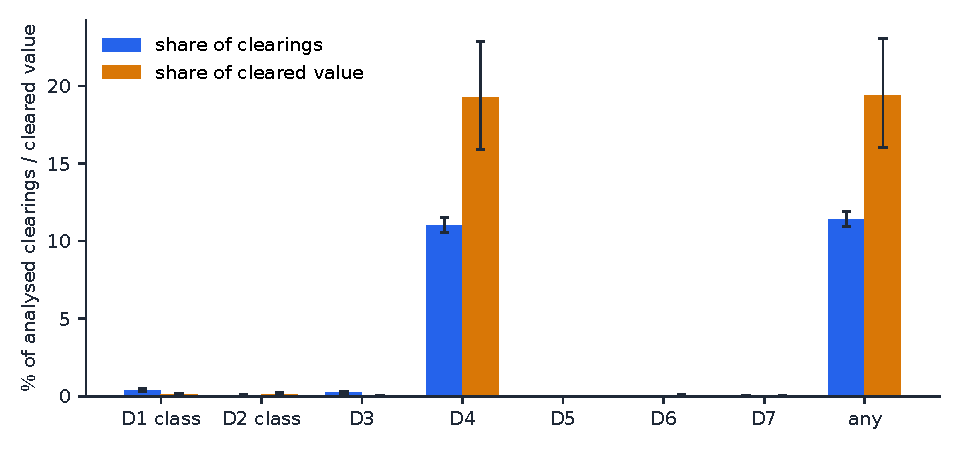
\includegraphics{../paper/figures/fig1-exposure.pdf}
\caption{Figure 1: share of analysed clearings and of cleared value per
defect class, with clustered bootstrap 95\% intervals.}
\end{figure}

\hypertarget{consequence-e2}{%
\subsubsection{5.2 Consequence (E2)}\label{consequence-e2}}

\begin{longtable}[]{@{}
  >{\raggedright\arraybackslash}p{(\columnwidth - 14\tabcolsep) * \real{0.1034}}
  >{\raggedright\arraybackslash}p{(\columnwidth - 14\tabcolsep) * \real{0.1034}}
  >{\raggedright\arraybackslash}p{(\columnwidth - 14\tabcolsep) * \real{0.1034}}
  >{\raggedleft\arraybackslash}p{(\columnwidth - 14\tabcolsep) * \real{0.1379}}
  >{\raggedleft\arraybackslash}p{(\columnwidth - 14\tabcolsep) * \real{0.1379}}
  >{\raggedleft\arraybackslash}p{(\columnwidth - 14\tabcolsep) * \real{0.1379}}
  >{\raggedleft\arraybackslash}p{(\columnwidth - 14\tabcolsep) * \real{0.1379}}
  >{\raggedleft\arraybackslash}p{(\columnwidth - 14\tabcolsep) * \real{0.1379}}@{}}
\toprule\noalign{}
\begin{minipage}[b]{\linewidth}\raggedright
test
\end{minipage} & \begin{minipage}[b]{\linewidth}\raggedright
defect group (failed predicate): O rate
\end{minipage} & \begin{minipage}[b]{\linewidth}\raggedright
comparison: O rate
\end{minipage} & \begin{minipage}[b]{\linewidth}\raggedleft
difference
\end{minipage} & \begin{minipage}[b]{\linewidth}\raggedleft
bootstrap SE
\end{minipage} & \begin{minipage}[b]{\linewidth}\raggedleft
z
\end{minipage} & \begin{minipage}[b]{\linewidth}\raggedleft
p (raw, one-sided)
\end{minipage} & \begin{minipage}[b]{\linewidth}\raggedleft
p (Holm)
\end{minipage} \\
\midrule\noalign{}
\endhead
\bottomrule\noalign{}
\endlastfoot
H1 & 39 of 692 (5.64\%) & 1,286 of 137,602 (0.93\%) & 0.0470 & 0.0127 &
3.688 & \(1.13 \times 10^{-4}\) & \(4.53 \times 10^{-4}\) \\
H2 & 327 of 17,157 (1.91\%) & 1,332 of 138,377 (0.96\%) & 0.0094 &
0.0018 & 5.266 & \(6.96 \times 10^{-8}\) & \(3.48 \times 10^{-7}\) \\
H3 & 0 of 0 (n/a) & 1,659 of 155,534 (1.07\%) & n/a & n/a & n/a & not
computable & 1 \\
\end{longtable}

O is the registered corrective within W = 60 days. The H1 comparison
group is three-way clearings with every applicable predicate passing;
against clearings of every category with every applicable predicate
passing the difference is 0.0470, descriptively. H2 compares D4 fail
with D4 pass in every category. Standard errors come from the
purchase-document-clustered bootstrap. Holm's adjustment runs over the
registered family of five tests, H1, H2, H3 and H4 for each model
family, at alpha = 0.05:

\begin{longtable}[]{@{}lrrrrl@{}}
\toprule\noalign{}
test & p (raw) & rank & multiplier & p (Holm) & below alpha \\
\midrule\noalign{}
\endhead
\bottomrule\noalign{}
\endlastfoot
H2 & \(6.96 \times 10^{-8}\) & 1 & 5 & \(3.48 \times 10^{-7}\) & yes \\
H1 & \(1.13 \times 10^{-4}\) & 2 & 4 & \(4.53 \times 10^{-4}\) & yes \\
H3 & 1 & 3 & 3 & 1 & no \\
H4-Haiku & 1 & 4 & 2 & 1 & no \\
H4-Jev & 1 & 5 & 1 & 1 & no \\
\end{longtable}

H3, distinct actors, is not computable: defect group has no analysed
clearings. No analysed clearing was made by an actor of its line's
earliest creation event, so the defect class has zero incidence; across
the log the actors who record a \texttt{Clear\ Invoice} and those who
record the earliest creation of a line are separate populations (23 and
185 actors, 0 in common; Section 6). No analysed clearing has D5 unknown
(0): the 7,941 \texttt{Clear\ Invoice} events with no actor all lie
outside the analysed set: of the 94 on framed lines, 94 fall after the
horizon T\_end - W (\texttt{results/e1/analysed-clearing-actors.json}).
H3 enters the family with p = 1, the convention the author fixed in
decision D-C-2, committed at 2026-10-25 18:21:56 UTC, before the first
model request at 2026-10-25 18:42:18 UTC
(\texttt{results/e4/timeline.json}). At W = 30 days the differences are
0.0354 for H1 and 0.0055 for H2, descriptively.

\hypertarget{gate-effect-and-hold-cost-e3}{%
\subsubsection{5.3 Gate effect and hold cost
(E3)}\label{gate-effect-and-hold-cost-e3}}

The gate would have held 17,748 of 155,534 analysed clearings (11.41\%,
19.41\% of cleared value); 0 of them were held on an unknown predicate
value alone. Against the corrective at W = 60 days, in clearings and
anonymised EUR (Figure 4):

\begin{longtable}[]{@{}lrr@{}}
\toprule\noalign{}
gate verdict & corrective within W & no corrective within W \\
\midrule\noalign{}
\endhead
\bottomrule\noalign{}
\endlastfoot
would have held & 368 (21,418,557) & 17,380 (145,068,897) \\
would have allowed & 1,291 (106,294,821) & 136,495 (584,977,346) \\
\end{longtable}

\begin{figure}
\centering
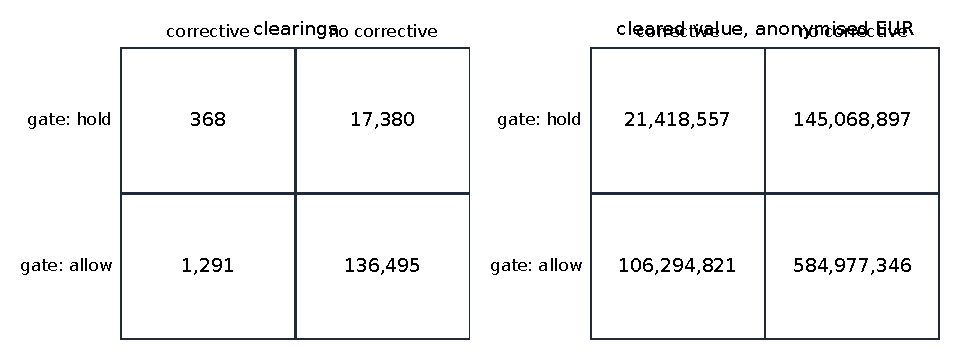
\includegraphics{../paper/figures/fig4-verdict-outcome.pdf}
\caption{Figure 4: gate verdict against the corrective within W = 60
days, in clearings and in cleared value.}
\end{figure}

For D1/D2 failures, the time from clearing to the first uncancelled
receipt (Figure 3):

\begin{longtable}[]{@{}lrr@{}}
\toprule\noalign{}
lag band & clearings & cleared value \\
\midrule\noalign{}
\endhead
\bottomrule\noalign{}
\endlastfoot
{[}0, 1{]} days & 11 & 109,886 \\
(1, 7{]} days & 21 & 113,119 \\
(7, 30{]} days & 11 & 803,512 \\
over 30 days & 39 & 44,240 \\
never (by T\_end) & 610 & 1,015,565 \\
\end{longtable}

\begin{figure}
\centering
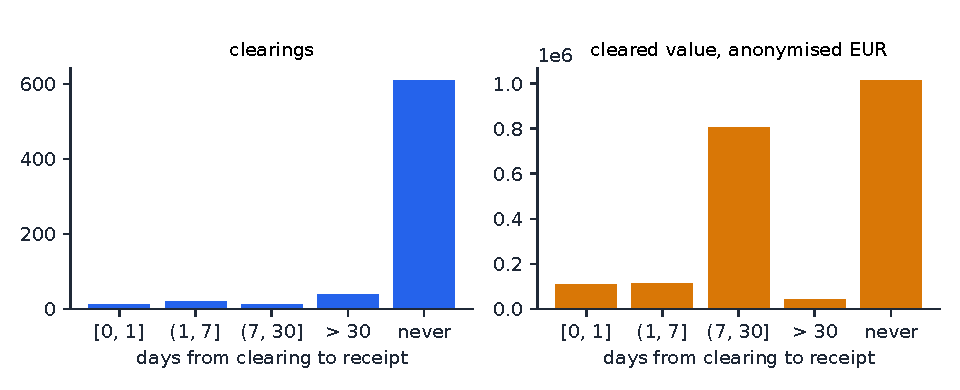
\includegraphics{../paper/figures/fig3-lag-bands.pdf}
\caption{Figure 3: D1/D2 failures by lag band, in clearings and cleared
value.}
\end{figure}

\textbf{Human hold.} Of 180,664 framed lines, people held 53,262 and
released 101,777; 25,625 had no invoice receipt by T\_end - W and are
not classified. The status of a line is the gate verdict at the decision
point t* of the agent replay: the first clearing if it came within W of
the first invoice receipt, otherwise that receipt plus W. The registered
text left D5 at a t* that is not a clearing undefined; read literally it
is unknown, and then a line with no clearing within W can never be clean
under the literal reading. The author amended the reading before any
model call (at a t* that is not a clearing, D5 is not applicable: the
decider there is the gate or a model; decision D-C-2 B); both readings
are reported:

\begin{longtable}[]{@{}
  >{\raggedright\arraybackslash}p{(\columnwidth - 8\tabcolsep) * \real{0.1667}}
  >{\raggedright\arraybackslash}p{(\columnwidth - 8\tabcolsep) * \real{0.1667}}
  >{\raggedleft\arraybackslash}p{(\columnwidth - 8\tabcolsep) * \real{0.2222}}
  >{\raggedleft\arraybackslash}p{(\columnwidth - 8\tabcolsep) * \real{0.2222}}
  >{\raggedleft\arraybackslash}p{(\columnwidth - 8\tabcolsep) * \real{0.2222}}@{}}
\toprule\noalign{}
\begin{minipage}[b]{\linewidth}\raggedright
reading
\end{minipage} & \begin{minipage}[b]{\linewidth}\raggedright
predicate status at t*
\end{minipage} & \begin{minipage}[b]{\linewidth}\raggedleft
classified lines
\end{minipage} & \begin{minipage}[b]{\linewidth}\raggedleft
held by people
\end{minipage} & \begin{minipage}[b]{\linewidth}\raggedleft
human hold rate
\end{minipage} \\
\midrule\noalign{}
\endhead
\bottomrule\noalign{}
\endlastfoot
literal (registered text) & defective & 16,264 & 5,664 & 34.83\% \\
literal (registered text) & clean & 91,178 & 1 & 0.00\% \\
literal (registered text) & held unknown & 47,597 & 47,597 & 100.00\% \\
amended (D-C-2 B) & defective & 16,264 & 5,664 & 34.83\% \\
amended (D-C-2 B) & clean & 138,775 & 47,598 & 34.30\% \\
amended (D-C-2 B) & held unknown & 0 & 0 & n/a \\
\end{longtable}

Under the amended reading, people held 34.83\% of lines with a failed
predicate at t* and 34.30\% of clean lines.

\hypertarget{people-models-and-the-gate-on-the-same-lines-e4}{%
\subsubsection{5.4 People, models and the gate on the same lines
(E4)}\label{people-models-and-the-gate-on-the-same-lines-e4}}

\textbf{Sample and arms.} From the framed lines with an invoice receipt,
18,006 had at least one failed predicate at t* and 147,240 were clean,
under D-C-2 B (\texttt{results/e4/sample-frame.json}). These differ from
the 16,264 and 138,775 lines of Section 5.3
(\texttt{results/e3/human-hold.json}), which are the lines the people
arm can classify: a line whose first invoice receipt comes later than
T\_end - W is eligible for the sample but not classified (section 3.6).
The registered sample drew 1,000 defective and 1,000 clean lines, at
most one per purchase document, stratified by category and value
quartile, with seed 20261201; the draw was committed before any call.
Each line was shown to two model families as the registered ERP view at
t*, a short record with no event timeline and no company, vendor, actor
or line id: TypeSafe System One (Jev, returned model
\texttt{jev-1.14.0}) through \texttt{typesafe-sdk==0.7.2}, asked one
choice question with labels clear and hold, and the Anthropic Messages
API (\texttt{claude-haiku-4-5-20251001}, temperature zero, assistant
prefill), asked for a JSON decision and hold probability. Invalid
replies, after one re-request: 0 for Jev and 0 for Haiku. The people arm
is read from the log (Section 3); 152 sample lines have no invoice
receipt by T\_end - W and are not classified (section 3.6), so its
denominators are smaller. The gate's verdict holds every line with a
failed predicate and allows every clean line by construction.

\begin{longtable}[]{@{}
  >{\raggedright\arraybackslash}p{(\columnwidth - 10\tabcolsep) * \real{0.1304}}
  >{\raggedleft\arraybackslash}p{(\columnwidth - 10\tabcolsep) * \real{0.1739}}
  >{\raggedleft\arraybackslash}p{(\columnwidth - 10\tabcolsep) * \real{0.1739}}
  >{\raggedleft\arraybackslash}p{(\columnwidth - 10\tabcolsep) * \real{0.1739}}
  >{\raggedleft\arraybackslash}p{(\columnwidth - 10\tabcolsep) * \real{0.1739}}
  >{\raggedleft\arraybackslash}p{(\columnwidth - 10\tabcolsep) * \real{0.1739}}@{}}
\toprule\noalign{}
\begin{minipage}[b]{\linewidth}\raggedright
arm
\end{minipage} & \begin{minipage}[b]{\linewidth}\raggedleft
held, lines with a failed predicate
\end{minipage} & \begin{minipage}[b]{\linewidth}\raggedleft
held, clean lines
\end{minipage} & \begin{minipage}[b]{\linewidth}\raggedleft
kappa with gate
\end{minipage} & \begin{minipage}[b]{\linewidth}\raggedleft
value released on lines with a failed predicate
\end{minipage} & \begin{minipage}[b]{\linewidth}\raggedleft
expected correctives
\end{minipage} \\
\midrule\noalign{}
\endhead
\bottomrule\noalign{}
\endlastfoot
people (from the log) & 301 of 912 (33.0\%) & 318 of 936 (34.0\%) & n/a
& 4,759,520 & 12.260 \\
Jev & 1,000 of 1,000 (100.0\%) & 530 of 1,000 (53.0\%) & 0.470 & 0 &
0.000 \\
Haiku & 996 of 1,000 (99.6\%) & 573 of 1,000 (57.3\%) & 0.423 & 7,307 &
0.076 \\
gate & 1,000 of 1,000 (100.0\%) & 0 of 1,000 (0.0\%) & n/a & 0 &
0.000 \\
\end{longtable}

\begin{longtable}[]{@{}
  >{\raggedright\arraybackslash}p{(\columnwidth - 10\tabcolsep) * \real{0.1304}}
  >{\raggedleft\arraybackslash}p{(\columnwidth - 10\tabcolsep) * \real{0.1739}}
  >{\raggedleft\arraybackslash}p{(\columnwidth - 10\tabcolsep) * \real{0.1739}}
  >{\raggedleft\arraybackslash}p{(\columnwidth - 10\tabcolsep) * \real{0.1739}}
  >{\raggedleft\arraybackslash}p{(\columnwidth - 10\tabcolsep) * \real{0.1739}}
  >{\raggedleft\arraybackslash}p{(\columnwidth - 10\tabcolsep) * \real{0.1739}}@{}}
\toprule\noalign{}
\begin{minipage}[b]{\linewidth}\raggedright
family
\end{minipage} & \begin{minipage}[b]{\linewidth}\raggedleft
d (failed predicate minus clean)
\end{minipage} & \begin{minipage}[b]{\linewidth}\raggedleft
SE
\end{minipage} & \begin{minipage}[b]{\linewidth}\raggedleft
p, lower
\end{minipage} & \begin{minipage}[b]{\linewidth}\raggedleft
p, upper
\end{minipage} & \begin{minipage}[b]{\linewidth}\raggedleft
p\_TOST
\end{minipage} \\
\midrule\noalign{}
\endhead
\bottomrule\noalign{}
\endlastfoot
H4-Jev & 0.470 & 0.0158 & \(2.33 \times 10^{-238}\) & 1 & 1 \\
H4-Haiku & 0.423 & 0.0158 & \(5.54 \times 10^{-198}\) & 1 & 1 \\
\end{longtable}

Source: \texttt{results/e4/arms.json}, \texttt{results/e4/h4.json}.

\begin{figure}
\centering
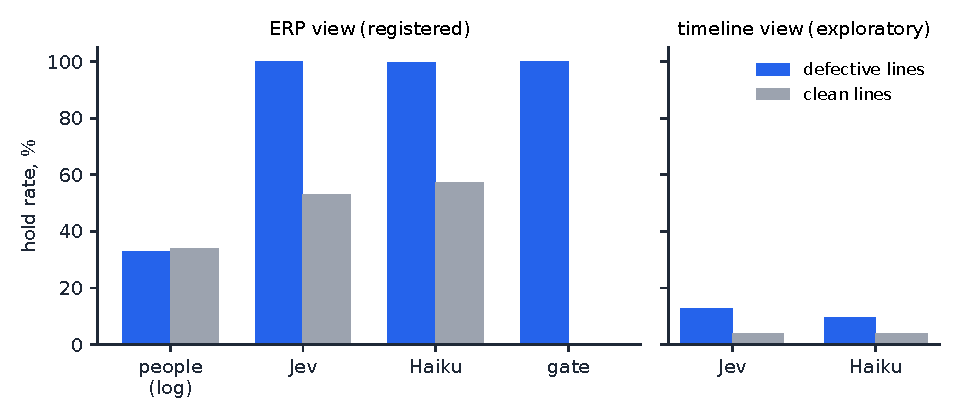
\includegraphics{../paper/figures/fig2-hold-rates.pdf}
\caption{Figure 2: hold rate on lines with a failed predicate and on
clean lines, per arm; the exploratory timeline arm in its own panel.}
\end{figure}

H4 asks whether each family's hold rate on defective lines (a failed
predicate) is within m = 0.05 of its rate on clean lines. Neither is:
Jev held 100.0\% and 53.0\%, Haiku held 99.6\% and 57.3\%; p\_TOST is 1
for Jev and 1 for Haiku, and H4 is below alpha after Holm for neither.
Both families track the gate's verdict on the lines the gate would have
held and hold about half of the lines it allows (Cohen's kappa with the
gate 0.470 and 0.423). Released on lines with a failed predicate, in
anonymised EUR: people 4,759,520, Jev 0, Haiku 7,307, gate 0; for the
gate, held lines go somewhere the log does not show. The expected
correctives are the metric of registration section 6 (E4 row): each
released line with a failed predicate carries the E2 O rate at W = 60
days of its defect group. The precedence and the unmatched-group rule
are decision D-C-3: the H1 group if D1/D2 fails and otherwise the H2
group if D4 fails; a line failing neither (only D3, D6 or D7) has no E2
group and is counted, not imputed (8 sample lines, 1 of them released by
people). The ERP view hands each model the inputs of the predicates;
this result is about the view as much as about the models.

\textbf{On the lines the people arm classifies.} The same four arms,
re-tabulated on the 1,848 sample lines the people arm classifies; the
table above, on all sample lines, stays primary:

\begin{longtable}[]{@{}
  >{\raggedright\arraybackslash}p{(\columnwidth - 10\tabcolsep) * \real{0.1304}}
  >{\raggedleft\arraybackslash}p{(\columnwidth - 10\tabcolsep) * \real{0.1739}}
  >{\raggedleft\arraybackslash}p{(\columnwidth - 10\tabcolsep) * \real{0.1739}}
  >{\raggedleft\arraybackslash}p{(\columnwidth - 10\tabcolsep) * \real{0.1739}}
  >{\raggedleft\arraybackslash}p{(\columnwidth - 10\tabcolsep) * \real{0.1739}}
  >{\raggedleft\arraybackslash}p{(\columnwidth - 10\tabcolsep) * \real{0.1739}}@{}}
\toprule\noalign{}
\begin{minipage}[b]{\linewidth}\raggedright
arm
\end{minipage} & \begin{minipage}[b]{\linewidth}\raggedleft
held, lines with a failed predicate
\end{minipage} & \begin{minipage}[b]{\linewidth}\raggedleft
held, clean lines
\end{minipage} & \begin{minipage}[b]{\linewidth}\raggedleft
kappa with gate
\end{minipage} & \begin{minipage}[b]{\linewidth}\raggedleft
value released on lines with a failed predicate
\end{minipage} & \begin{minipage}[b]{\linewidth}\raggedleft
expected correctives
\end{minipage} \\
\midrule\noalign{}
\endhead
\bottomrule\noalign{}
\endlastfoot
people (from the log) & 301 of 912 (33.0\%) & 318 of 936 (34.0\%) & n/a
& 4,759,520 & 12.260 \\
Jev & 912 of 912 (100.0\%) & 491 of 936 (52.5\%) & 0.472 & 0 & 0.000 \\
Haiku & 908 of 912 (99.6\%) & 524 of 936 (56.0\%) & 0.433 & 7,307 &
0.076 \\
gate & 912 of 912 (100.0\%) & 0 of 936 (0.0\%) & n/a & 0 & 0.000 \\
\end{longtable}

Source: \texttt{results/e4/arms-classified-lines.json}; a re-tabulation
on the lines the people arm classifies.

\textbf{What the people arm measures.} The log records no hold decision
except a payment block. ``Held by people'' (section 3.6) is a payment
block before the first clearing, or no clearing within W of the first
invoice receipt: an inferred non-release, not the same act as a model's
hold verdict at t*. Of the 53,262 framed lines held by people, 10 were
held by a payment block alone, 53,182 by no clearing within W alone, and
70 by both:

\begin{longtable}[]{@{}
  >{\raggedright\arraybackslash}p{(\columnwidth - 10\tabcolsep) * \real{0.1364}}
  >{\raggedright\arraybackslash}p{(\columnwidth - 10\tabcolsep) * \real{0.1364}}
  >{\raggedleft\arraybackslash}p{(\columnwidth - 10\tabcolsep) * \real{0.1818}}
  >{\raggedleft\arraybackslash}p{(\columnwidth - 10\tabcolsep) * \real{0.1818}}
  >{\raggedleft\arraybackslash}p{(\columnwidth - 10\tabcolsep) * \real{0.1818}}
  >{\raggedleft\arraybackslash}p{(\columnwidth - 10\tabcolsep) * \real{0.1818}}@{}}
\toprule\noalign{}
\begin{minipage}[b]{\linewidth}\raggedright
reading
\end{minipage} & \begin{minipage}[b]{\linewidth}\raggedright
predicate status at t*
\end{minipage} & \begin{minipage}[b]{\linewidth}\raggedleft
held by people
\end{minipage} & \begin{minipage}[b]{\linewidth}\raggedleft
payment block before the first clearing
\end{minipage} & \begin{minipage}[b]{\linewidth}\raggedleft
no clearing within W of the first invoice
\end{minipage} & \begin{minipage}[b]{\linewidth}\raggedleft
both
\end{minipage} \\
\midrule\noalign{}
\endhead
\bottomrule\noalign{}
\endlastfoot
literal (registered text) & defective & 5,664 & 9 & 5,619 & 36 \\
literal (registered text) & clean & 1 & 1 & 0 & 0 \\
literal (registered text) & held unknown & 47,597 & 0 & 47,563 & 34 \\
amended (D-C-2 B) & defective & 5,664 & 9 & 5,619 & 36 \\
amended (D-C-2 B) & clean & 47,598 & 1 & 47,563 & 34 \\
amended (D-C-2 B) & held unknown & 0 & 0 & 0 & 0 \\
\end{longtable}

Source: \texttt{results/e3/human-hold-composition.json}.

\textbf{Exploratory: the event timeline instead of the ERP view.}
Labelled exploratory and outside the Holm family: the same lines, the
same families and rules, with the line's events up to t* (date,
activity, value) in place of the ERP view.

\begin{longtable}[]{@{}
  >{\raggedright\arraybackslash}p{(\columnwidth - 8\tabcolsep) * \real{0.1579}}
  >{\raggedleft\arraybackslash}p{(\columnwidth - 8\tabcolsep) * \real{0.2105}}
  >{\raggedleft\arraybackslash}p{(\columnwidth - 8\tabcolsep) * \real{0.2105}}
  >{\raggedleft\arraybackslash}p{(\columnwidth - 8\tabcolsep) * \real{0.2105}}
  >{\raggedleft\arraybackslash}p{(\columnwidth - 8\tabcolsep) * \real{0.2105}}@{}}
\toprule\noalign{}
\begin{minipage}[b]{\linewidth}\raggedright
family (timeline view, exploratory)
\end{minipage} & \begin{minipage}[b]{\linewidth}\raggedleft
held, lines with a failed predicate
\end{minipage} & \begin{minipage}[b]{\linewidth}\raggedleft
held, clean lines
\end{minipage} & \begin{minipage}[b]{\linewidth}\raggedleft
kappa with gate
\end{minipage} & \begin{minipage}[b]{\linewidth}\raggedleft
invalid replies
\end{minipage} \\
\midrule\noalign{}
\endhead
\bottomrule\noalign{}
\endlastfoot
Jev & 126 of 1,000 (12.6\%) & 38 of 1,000 (3.8\%) & 0.088 & 0 \\
Haiku & 95 of 1,000 (9.5\%) & 39 of 1,000 (3.9\%) & 0.056 & 0 \\
\end{longtable}

Source: \texttt{results/e4-exploratory/arms-exploratory.json};
exploratory, no interval, outside the Holm family.

Under the timeline view the same models held far fewer lines with a
failed predicate (exploratory, no interval). Spend for both families and
both views together was USD 1.57 against the registered cap of USD 60
(\texttt{results/e6/cost.json}).

\hypertarget{derivation-e5}{%
\subsubsection{5.5 Derivation (E5)}\label{derivation-e5}}

Paper 5's compiler, at the pinned commit and unmodified, was given per
category the observed states of the evidence set and the three declared
losses of the registration: L1, pay for goods not received (the category
requires a goods receipt and none is uncancelled); L2, pay twice (the
clearing's position among the line's clearings exceeds the invoices
recorded); L3, pay a changed amount (a change since approval). The
derived contract is the set of registered predicates whose observation
is in the compiler's minimum-cardinality sufficient set. The comparison
is the registered one (registration section 6, E5): ``whether the
derived contract equals the category contract in 3.1''.

\begin{longtable}[]{@{}
  >{\raggedright\arraybackslash}p{(\columnwidth - 18\tabcolsep) * \real{0.0857}}
  >{\raggedleft\arraybackslash}p{(\columnwidth - 18\tabcolsep) * \real{0.1143}}
  >{\raggedleft\arraybackslash}p{(\columnwidth - 18\tabcolsep) * \real{0.1143}}
  >{\raggedleft\arraybackslash}p{(\columnwidth - 18\tabcolsep) * \real{0.1143}}
  >{\raggedleft\arraybackslash}p{(\columnwidth - 18\tabcolsep) * \real{0.1143}}
  >{\raggedleft\arraybackslash}p{(\columnwidth - 18\tabcolsep) * \real{0.1143}}
  >{\raggedright\arraybackslash}p{(\columnwidth - 18\tabcolsep) * \real{0.0857}}
  >{\raggedright\arraybackslash}p{(\columnwidth - 18\tabcolsep) * \real{0.0857}}
  >{\raggedright\arraybackslash}p{(\columnwidth - 18\tabcolsep) * \real{0.0857}}
  >{\raggedright\arraybackslash}p{(\columnwidth - 18\tabcolsep) * \real{0.0857}}@{}}
\toprule\noalign{}
\begin{minipage}[b]{\linewidth}\raggedright
category
\end{minipage} & \begin{minipage}[b]{\linewidth}\raggedleft
clearings
\end{minipage} & \begin{minipage}[b]{\linewidth}\raggedleft
states
\end{minipage} & \begin{minipage}[b]{\linewidth}\raggedleft
L1
\end{minipage} & \begin{minipage}[b]{\linewidth}\raggedleft
L2
\end{minipage} & \begin{minipage}[b]{\linewidth}\raggedleft
L3
\end{minipage} & \begin{minipage}[b]{\linewidth}\raggedright
fewest fields
\end{minipage} & \begin{minipage}[b]{\linewidth}\raggedright
derived contract
\end{minipage} & \begin{minipage}[b]{\linewidth}\raggedright
registered contract
\end{minipage} & \begin{minipage}[b]{\linewidth}\raggedright
result
\end{minipage} \\
\midrule\noalign{}
\endhead
\bottomrule\noalign{}
\endlastfoot
2-way & 188 & 3 & 0 & 0 & 4 & \texttt{changes} & D4 & D3, D4, D5, D6, D7
& does not reproduce \\
3-way, invoice after receipt & 9,640 & 896 & 0 & 81 & 1,585 &
\texttt{changes}, \texttt{clearing\_ordinal}, \texttt{invoices} & D3, D4
& D1, D2, D3, D4, D5, D6, D7 & does not reproduce \\
3-way, invoice before receipt & 145,706 & 758 & 692 & 1,390 & 15,568 &
\texttt{changes}, \texttt{clearing\_ordinal}, \texttt{invoices},
\texttt{receipts} & D1, D2, D3, D4 & D1, D2, D3, D4, D5, D6, D7 & does
not reproduce \\
\end{longtable}

The compiler does not reproduce the registered contract in any category.
The three losses derive at most D1 to D4: no declared loss reads the
observations of D5, D6 or D7, so those predicates correspond to no
declared loss. In the before-receipt category the derived D1 to D4 is
the three-way match in the narrow sense (receipt, invoice and an
unchanged approved amount), and the registered contract carries three
predicates beyond it. In the after-receipt category the compiler derives
D3 and D4 only, because L1 occurs on 0 analysed clearings there, and the
registered contract carries five predicates beyond it. This is a limit
of deriving from one log: a loss the log never shows calls for no
observation. Pay twice needs the clearing's position on its line, an
observation no registered predicate reads.

Read the other way, paper 5's sufficiency function applied to the
registered contract over the same states
(\texttt{results/e5/sufficiency.json}):

\begin{longtable}[]{@{}
  >{\raggedright\arraybackslash}p{(\columnwidth - 12\tabcolsep) * \real{0.1364}}
  >{\raggedright\arraybackslash}p{(\columnwidth - 12\tabcolsep) * \real{0.1364}}
  >{\raggedright\arraybackslash}p{(\columnwidth - 12\tabcolsep) * \real{0.1364}}
  >{\raggedright\arraybackslash}p{(\columnwidth - 12\tabcolsep) * \real{0.1364}}
  >{\raggedleft\arraybackslash}p{(\columnwidth - 12\tabcolsep) * \real{0.1818}}
  >{\raggedright\arraybackslash}p{(\columnwidth - 12\tabcolsep) * \real{0.1364}}
  >{\raggedright\arraybackslash}p{(\columnwidth - 12\tabcolsep) * \real{0.1364}}@{}}
\toprule\noalign{}
\begin{minipage}[b]{\linewidth}\raggedright
category
\end{minipage} & \begin{minipage}[b]{\linewidth}\raggedright
registered fields
\end{minipage} & \begin{minipage}[b]{\linewidth}\raggedright
sufficient for
\end{minipage} & \begin{minipage}[b]{\linewidth}\raggedright
not sufficient for
\end{minipage} & \begin{minipage}[b]{\linewidth}\raggedleft
clearings with L2
\end{minipage} & \begin{minipage}[b]{\linewidth}\raggedright
minimal
\end{minipage} & \begin{minipage}[b]{\linewidth}\raggedright
derived contract a subset
\end{minipage} \\
\midrule\noalign{}
\endhead
\bottomrule\noalign{}
\endlastfoot
2-way & \texttt{invoices}, \texttt{changes}, \texttt{distinct\_actors},
\texttt{blocks}, \texttt{closed} & L1, L2, L3 & none & 0 & no & yes \\
3-way, invoice after receipt & \texttt{receipts}, \texttt{invoices},
\texttt{changes}, \texttt{distinct\_actors}, \texttt{blocks},
\texttt{closed} & L1, L3 & L2 & 81 & no & yes \\
3-way, invoice before receipt & \texttt{receipts}, \texttt{invoices},
\texttt{changes}, \texttt{distinct\_actors}, \texttt{blocks},
\texttt{closed} & L1, L3 & L2 & 1,390 & no & yes \\
\end{longtable}

The registered contract is sufficient, not derived: sufficient for the
three declared losses in the two-way category, and in the three-way
categories for L1 and L3 but not for L2, for the reason above; minimal
in no category (C1). The compiler's contract is smaller in every
category, and so C9, which asks whether it equals the registered one, is
not supported.

\hypertarget{governance-cost-e6}{%
\subsubsection{5.6 Governance cost (E6)}\label{governance-cost-e6}}

The full replay of every line, from reading the log to the written
evidence set, took a median of 153.5 seconds over three runs on a 4-core
machine, 0.000987 seconds per gate decision. A model decision cost USD
0.000022 with Jev and USD 0.000368 with Haiku.

\hypertarget{replication-on-travel-declarations-e7}{%
\subsubsection{5.7 Replication on travel declarations
(E7)}\label{replication-on-travel-declarations-e7}}

The unit is a payment on a declaration case at least W before the latest
timestamp of its log; D1' approval present, D2' approval by the required
role and D3' unchanged after approval are evaluated before the payment,
and O' is a rejection or resubmission within W after it. Descriptive and
secondary, outside the Holm family.

\begin{longtable}[]{@{}lrrrr@{}}
\toprule\noalign{}
log & cases & payments & excluded after T\_end' - W & units \\
\midrule\noalign{}
\endhead
\bottomrule\noalign{}
\endlastfoot
domestic & 10,500 & 10,044 & 2 & 10,042 \\
international & 6,449 & 6,187 & 0 & 6,187 \\
\end{longtable}

\begin{longtable}[]{@{}
  >{\raggedright\arraybackslash}p{(\columnwidth - 12\tabcolsep) * \real{0.1200}}
  >{\raggedright\arraybackslash}p{(\columnwidth - 12\tabcolsep) * \real{0.1200}}
  >{\raggedleft\arraybackslash}p{(\columnwidth - 12\tabcolsep) * \real{0.1600}}
  >{\raggedleft\arraybackslash}p{(\columnwidth - 12\tabcolsep) * \real{0.1600}}
  >{\raggedleft\arraybackslash}p{(\columnwidth - 12\tabcolsep) * \real{0.1600}}
  >{\raggedleft\arraybackslash}p{(\columnwidth - 12\tabcolsep) * \real{0.1600}}
  >{\raggedright\arraybackslash}p{(\columnwidth - 12\tabcolsep) * \real{0.1200}}@{}}
\toprule\noalign{}
\begin{minipage}[b]{\linewidth}\raggedright
scope
\end{minipage} & \begin{minipage}[b]{\linewidth}\raggedright
predicate
\end{minipage} & \begin{minipage}[b]{\linewidth}\raggedleft
failing payments
\end{minipage} & \begin{minipage}[b]{\linewidth}\raggedleft
O' rate, failing
\end{minipage} & \begin{minipage}[b]{\linewidth}\raggedleft
O' rate, all-pass
\end{minipage} & \begin{minipage}[b]{\linewidth}\raggedleft
difference
\end{minipage} & \begin{minipage}[b]{\linewidth}\raggedright
bootstrap 95\%
\end{minipage} \\
\midrule\noalign{}
\endhead
\bottomrule\noalign{}
\endlastfoot
domestic & D1' & 2 & 0.500 & 0.000 & 0.500 & {[}0.0000, 1.0000{]} \\
domestic & D2' & 2 & 0.500 & 0.000 & 0.500 & {[}0.0000, 1.0000{]} \\
domestic & D3' & 0 & n/a & 0.000 & n/a & n/a \\
international & D1' & 0 & n/a & 0.000 & n/a & n/a \\
international & D2' & 0 & n/a & 0.000 & n/a & n/a \\
international & D3' & 0 & n/a & 0.000 & n/a & n/a \\
pooled & D1' & 2 & 0.500 & 0.000 & 0.500 & {[}0.0000, 1.0000{]} \\
pooled & D2' & 2 & 0.500 & 0.000 & 0.500 & {[}0.0000, 1.0000{]} \\
pooled & D3' & 0 & n/a & 0.000 & n/a & n/a \\
\end{longtable}

The replication is inconclusive. Only 2 of 16,229 payments fail any
predicate; the 2 domestic payments with D3' unknown are the same 2 that
fail D1' and D2' (\texttt{results/e7/unknown-overlap.json}). O' follows
0 of the 16,227 payments with every predicate passing; no comparison has
an interval excluding zero. A bootstrap replicate in which either group
is empty is discarded and the percentiles are taken over the retained
replicates (8,685 of 10,000 for the domestic log and 8,696 pooled,
\texttt{results/e7/comparisons.json}; a deviation, Section 4). The
registered names \texttt{Declaration\ FINAL\_APPROVED\ by\ DIRECTOR} and
\texttt{Declaration\ REJECTED\ by\ DIRECTOR} do not occur in the
domestic log; they are reported with zero counts, not replaced.

\hypertarget{coverage}{%
\subsection{6 Coverage}\label{coverage}}

What the replay can and cannot see, as registered:

\textbf{Detected (BPI 2019, E1 to E6)}

\begin{longtable}[]{@{}
  >{\raggedright\arraybackslash}p{(\columnwidth - 6\tabcolsep) * \real{0.2500}}
  >{\raggedright\arraybackslash}p{(\columnwidth - 6\tabcolsep) * \real{0.2500}}
  >{\raggedright\arraybackslash}p{(\columnwidth - 6\tabcolsep) * \real{0.2500}}
  >{\raggedright\arraybackslash}p{(\columnwidth - 6\tabcolsep) * \real{0.2500}}@{}}
\toprule\noalign{}
\begin{minipage}[b]{\linewidth}\raggedright
defect class
\end{minipage} & \begin{minipage}[b]{\linewidth}\raggedright
predicate
\end{minipage} & \begin{minipage}[b]{\linewidth}\raggedright
dimension
\end{minipage} & \begin{minipage}[b]{\linewidth}\raggedright
detected from
\end{minipage} \\
\midrule\noalign{}
\endhead
\bottomrule\noalign{}
\endlastfoot
goods receipt required but absent at clearing & D1 receipt\_present &
presence & receipts minus cancellations at most zero before t\_c (count
of \texttt{Record\ Goods\ Receipt} minus count of
\texttt{Cancel\ Goods\ Receipt}), on a line whose category requires
receipt \\
stale receipt: receipt recorded after clearing & D2
receipt\_before\_clearing & freshness, order & the first uncancelled
\texttt{Record\ Goods\ Receipt} falls after t\_c (lag band
registered) \\
invoice absent at clearing & D3 invoice\_present & presence & no
\texttt{Record\ Invoice\ Receipt} before t\_c \\
changed after approval & D4 unchanged\_since\_approval & validity &
\texttt{Change\ Price} or \texttt{Change\ Quantity} between the last
approval-bearing event and t\_c \\
same actor created and cleared & D5 distinct\_actors & authority & actor
of \texttt{Create\ Purchase\ Order\ Item} equals actor of
\texttt{Clear\ Invoice} \\
clearing under an open payment block & D6 block\_respected & scope &
count of \texttt{Set\ Payment\ Block} minus count of
\texttt{Remove\ Payment\ Block} before t\_c greater than zero \\
line deleted or blocked at clearing & D7 not\_deleted & validity & count
of \texttt{Delete\ Purchase\ Order\ Item} plus
\texttt{Block\ Purchase\ Order\ Item} minus
\texttt{Reactivate\ Purchase\ Order\ Item} before t\_c greater than
zero \\
\end{longtable}

\textbf{Detected (BPI 2020 declarations, E7, secondary)}

\begin{longtable}[]{@{}
  >{\raggedright\arraybackslash}p{(\columnwidth - 6\tabcolsep) * \real{0.2500}}
  >{\raggedright\arraybackslash}p{(\columnwidth - 6\tabcolsep) * \real{0.2500}}
  >{\raggedright\arraybackslash}p{(\columnwidth - 6\tabcolsep) * \real{0.2500}}
  >{\raggedright\arraybackslash}p{(\columnwidth - 6\tabcolsep) * \real{0.2500}}@{}}
\toprule\noalign{}
\begin{minipage}[b]{\linewidth}\raggedright
defect class
\end{minipage} & \begin{minipage}[b]{\linewidth}\raggedright
predicate
\end{minipage} & \begin{minipage}[b]{\linewidth}\raggedright
dimension
\end{minipage} & \begin{minipage}[b]{\linewidth}\raggedright
detected from
\end{minipage} \\
\midrule\noalign{}
\endhead
\bottomrule\noalign{}
\endlastfoot
paid without an approval event & D1' approval\_present & presence & no
event in the registered approval list before the payment \\
approved by a role other than the required one & D2'
approval\_by\_required\_role & authority & the approval chain before
payment lacks the registered required role \\
declaration changed after approval & D3' unchanged\_since\_approval &
validity & a resubmission by the employee between the last approval and
payment \\
\end{longtable}

\textbf{Undetected, with reason}

\begin{longtable}[]{@{}
  >{\raggedright\arraybackslash}p{(\columnwidth - 2\tabcolsep) * \real{0.5000}}
  >{\raggedright\arraybackslash}p{(\columnwidth - 2\tabcolsep) * \real{0.5000}}@{}}
\toprule\noalign{}
\begin{minipage}[b]{\linewidth}\raggedright
defect class
\end{minipage} & \begin{minipage}[b]{\linewidth}\raggedright
reason
\end{minipage} \\
\midrule\noalign{}
\endhead
\bottomrule\noalign{}
\endlastfoot
wrong amounts in the payload & values are anonymised by a linear
translation; the log carries cumulative net worth per event, not invoice
line content, so a mismatch between invoice text and goods is not
observable \\
fraud & intent is not an event attribute; no predicate over the log
separates a fraudulent clearing from an erroneous one, and the paper
makes no statement about it \\
vendor identity (wrong, duplicate or fictitious vendor) & vendor names
and ids are anonymised consistently; the log carries no master-data
change history or bank details \\
recovery of corrected payments & the log records the corrective event
and nothing about recovery; whether money was returned, offset or
written off is not recorded \\
what a held line becomes & a gate hold is a replay verdict; the log
records the human path only, so the fate of a line the gate would have
held is not observable \\
approvals outside the log & approvals given by e-mail, in another system
or verbally leave no event; D4's ``last approval-bearing event'' sees
only logged approvals \\
partial receipt and value mismatch per receipt & the replay checks
presence and order of the receipt, not the matched values; values are
anonymised and the registered mapping reads no per-receipt quantity \\
duplicate invoice across lines & the case is one purchase-order line and
the registered mapping carries no invoice document id, so an invoice
cleared on two lines is not linked \\
\end{longtable}

Per class, the failures found (BPI 2019 on analysed clearings, BPI 2020
on payments):

\begin{longtable}[]{@{}llrr@{}}
\toprule\noalign{}
log & predicate & failed & unknown \\
\midrule\noalign{}
\endhead
\bottomrule\noalign{}
\endlastfoot
BPI 2019 (analysed clearings) & D1 & 692 & n/a \\
BPI 2019 (analysed clearings) & D2 & 692 & n/a \\
BPI 2019 (analysed clearings) & D3 & 362 & n/a \\
BPI 2019 (analysed clearings) & D4 & 17,157 & n/a \\
BPI 2019 (analysed clearings) & D5 & 0 & 0 \\
BPI 2019 (analysed clearings) & D6 & 4 & n/a \\
BPI 2019 (analysed clearings) & D7 & 19 & n/a \\
BPI 2020 domestic (payments) & D1' & 2 & 0 \\
BPI 2020 domestic (payments) & D2' & 2 & 0 \\
BPI 2020 domestic (payments) & D3' & 0 & 2 \\
BPI 2020 international (payments) & D1' & 0 & 0 \\
BPI 2020 international (payments) & D2' & 0 & 0 \\
BPI 2020 international (payments) & D3' & 0 & 0 \\
\end{longtable}

Sources: \texttt{results/e1/coverage-check.json},
\texttt{results/e1/analysed-clearing-actors.json} (D5 unknown),
\texttt{results/e7/predicates.json}.

On BPI 2019 every detected class fails at least once except the
authority class (D5), with 0 failed clearings: across the log, the 23
actors who record a \texttt{Clear\ Invoice} and the 185 who record a
line's earliest creation share 0, so the two are separate populations;
no \texttt{Clear\ Invoice} is recorded by a batch user (an actor whose
name starts with the registered batch prefix), and 7,941 carry no actor
(\texttt{results/e1/actors.json}), none of them on an analysed clearing
(0; Section 5.2). D5 fires on synthetic lines in the engine's tests
(\texttt{test\_d5\_actors} and
\texttt{test\_verdict\_at\_decision\_point\_d5\_off\_clearing} in
\texttt{tests/test\_engine\_units.py}, and fixture line C in
\texttt{tests/test\_pipeline.py}). On BPI 2020, D3' fails on no payment
in either log, and in the international log no predicate fails at all.

\hypertarget{limitations-and-non-claims}{%
\subsection{7 Limitations and
non-claims}\label{limitations-and-non-claims}}

The outcome is a proxy: a corrective event after a clearing is not proof
that the clearing was wrong, and the study is observational. Category,
spend area, value, vendor activity and month are reported beside every
estimate and never modelled in. Values are anonymised. What a line the
gate would have held becomes is not in the log. The people column
reports what the process did within W; the comparison across the people,
the models and the gate is of outcomes of three deciders, not of three
acts. The ERP view hands the model the inputs of the predicates; under
the timeline view the same models held far fewer lines (exploratory, no
interval), which is a statement about views, not about the models alone.
The derivation depends on how the three declared losses are expressed
over the evidence set; the expressions are recorded with the result. One
company's process, one year.

\hypertarget{conclusion}{%
\subsection{8 Conclusion}\label{conclusion}}

11.41\% of the 155,534 analysed invoice clearings in this process were
made on evidence that failed at least one registered predicate, carrying
19.41\% of the cleared value; those made with an absent or late receipt
(D1/D2) were followed by a corrective at a higher rate than three-way
clearings with every applicable predicate passing, and those made after
a change since approval (D4 fail) at a higher rate than D4-pass
clearings.

\hypertarget{acknowledgements}{%
\subsection{Acknowledgements}\label{acknowledgements}}

The prior-art fence was reviewed externally by Eduardo Arana after the
tag \texttt{prereg-p7-v1} and before \texttt{prereg-p7-v1.1}, and he
reviewed drafts v0.1 and v0.2. AI tools were used as support: builder
sessions with Claude for the code, the runs and the drafting from slots;
two machine prior-art sweeps, on ChatGPT and on Perplexity Computer (for
the second, the platform made two statements, in this order: a later
session reported its own model as \texttt{Claude\ Opus\ 5.5} and stated
that it produced the sweep, and the same session then identified the
sweep's model as \texttt{DeepSeek\ V4\ Pro}); and machine reviews of
drafts v0.1 and v0.2, on ChatGPT and on Perplexity Computer (model as it
states it: \texttt{Claude\ Opus\ 5.5}). All are committed unedited. The
author is solely responsible for every claim. We thank the organisers of
the BPI Challenges and 4TU.ResearchData for the logs.

\hypertarget{references}{%
\subsection{References}\label{references}}

\begin{itemize}
\item
  Peyman Badakhshan, Samuel Gosling, Jerome Geyer-Klingeberg, Janina
  Nakladal, Johannes Schukat, Jennifer Gsenger (2019). Process Mining in
  the Coatings and Paints Industry: The Purchase Order Handling Process.
  BPI Challenge 2019 report, non-student category, ICPM 2019.
  https://icpmconference.org/2019/wp-content/uploads/sites/6/2019/07/BPI-Challenge-Submission-4.pdf
\item
  Gaston Besanson (2026a). One Gate Is Not Enough: Composing Stateful
  Pre-Action Controls for Agentic AI. arXiv:2608.18360 (paper 4 of the
  SARC series; repository sarc-suite-one-pass).
  https://arxiv.org/abs/2608.18360
\item
  Gaston Besanson (2026b). Compiling Sufficient Governance Context from
  Declared Losses and Reachable States: Exact Observation-Contract
  Synthesis with Cardinality and Cost Objectives. arXiv:2609.26016
  (paper 5 of this programme; CITATION.cff of
  sarc-authority-derivation). https://arxiv.org/pdf/2609.26016
\item
  Gaston Besanson (2026c). gigo-jev-probe: a preregistered probe of a
  model as an advisory data-quality critic (paper 6 of the SARC series).
  public GitHub repository besanson/gigo-jev-probe, pinned in
  engines.lock at e1fc75b. https://github.com/besanson/gigo-jev-probe
\item
  Kiarash Diba, Simon Remy, Luise Pufahl (2019). BPI Challenge 2019:
  Performance and Compliance Analysis of Procurement Processes Using
  Process Mining. BPI Challenge 2019 report, non-student category, ICPM
  2019.
  https://icpmconference.org/2019/wp-content/uploads/sites/6/2019/07/BPI-Challenge-Submission-6.pdf
\item
  Matthew Harding, Gabriel F. R. Vasconcelos (2022). Managers versus
  Machines: Do Algorithms Replicate Human Intuition in Credit Ratings?.
  arXiv:2202.04218 (submitted 2022-02-09).
  https://arxiv.org/abs/2202.04218
\item
  ICPM 2019 (2019). BPI Challenge 2019 (ICPM 2019 conference page).
  https://icpmconference.org/2019/bpi-challenge/
\item
  ICPM 2020 (2020a). Awards (ICPM 2020).
  https://icpmconference.org/2020/awards/
\item
  ICPM 2020 (2020b). BPI Challenge 2020 (ICPM 2020 conference page).
  https://icpmconference.org/2020/bpi-challenge/
\item
  Md Abdul Kadir, Sai Suresh Macharla Vasu, Sidharth S. Nair, Daniel
  Sonntag (2025). AuditCopilot: Leveraging LLMs for Fraud Detection in
  Double-Entry Bookkeeping. arXiv:2512.02726 (submitted 2025-12-02).
  https://arxiv.org/abs/2512.02726
\item
  Stijn Kas, Ruben Post, Sebastiaan Wiewel (2020). Automated Machine
  Learning in a Process Mining Context. BPI Student Challenge Award,
  ICPM 2020.
  https://icpmconference.org/2020/wp-content/uploads/sites/4/2020/10/ICPM\_2020\_paper\_44.pdf
\item
  Linh Thao Ly, Fabrizio Maria Maggi, Marco Montali, Stefanie
  Rinderle-Ma, Wil M.P. van der Aalst (2015). Compliance monitoring in
  business processes: Functionalities, application, and tool-support.
  Information Systems 54, 209-234 (December 2015), Elsevier.
  doi:10.1016/j.is.2015.02.007
\item
  Vincent Finn Alexander Meyer zu Wickern, Mounisha Juluru, Anshu Roy,
  Viet-Hung Vu, Thi-Thu-Hang Nguyen (2019). Analysis and prediction of
  purchasing compliance using process mining. BPI Challenge 2019 report,
  student category, ICPM 2019.
  https://icpmconference.org/2019/wp-content/uploads/sites/6/2019/07/BPI-Challenge-Student-Submission-4.pdf
\item
  Hoang Nguyen, Marlon Dumas, Marcello La Rosa, Fabrizio Maria Maggi,
  Suriadi Suriadi (2016). Business Process Deviance Mining: Review and
  Evaluation. arXiv:1608.08252 (submitted 2016-08-29).
  https://arxiv.org/abs/1608.08252
\item
  Nesi Outmazgin, Pnina Soffer (2013). Business Process Workarounds:
  What Can and Cannot Be Detected by Process Mining. Enterprise,
  Business-Process and Information Systems Modeling (BPMDS 2013, EMMSAD
  2013), LNBIP vol.~147, pp.~48-62, Springer.
  doi:10.1007/978-3-642-38484-4\_5
\item
  Diego Palma, Kyu Bin Kim, Zhen Han, Allbright Dsouza, Zhiyuan Liu
  (2026). Business Compromise Detection with Agentic AI and LLM-driven
  Knowledge Discovery. arXiv:2609.32643 (submitted 2026-09-26).
  https://arxiv.org/html/2609.32643
\item
  Public Company Accounting Oversight Board (2004). An Audit of Internal
  Control Over Financial Reporting Performed in Conjunction with an
  Audit of Financial Statements (PCAOB Release No.~2004-001). PCAOB
  Release 2004-001, March 9, 2004.
  https://pcaobus.org/Rulemaking/Docket008/2004-03-09\_Release\_2004-001-all.pdf
\item
  Mor Peleg, Pnina Soffer, Johny Ghattas (2008). Mining Process
  Execution and Outcomes -- Position Paper. Business Process Management
  Workshops (BPM 2007), LNCS vol.~4928, pp.~395-400, Springer.
  doi:10.1007/978-3-540-78238-4\_40
\item
  Maja Pesic, Helen Schonenberg, Wil M.P. van der Aalst (2007). DECLARE:
  Full Support for Loosely-Structured Processes. 11th IEEE International
  Enterprise Distributed Object Computing Conference (EDOC 2007),
  p.~287, IEEE. doi:10.1109/EDOC.2007.14
\item
  Adrien Porter, David Masse, Nuss Visatemongkolchai, Jithendra
  Seneviratne, Tanvee Deokule, Nicholas Hartman (2019). Balancing
  Efficiency and Risk in Procure to Pay: Safely Realizing Cost Savings
  Using Process Mining Techniques. BPI Challenge 2019 report,
  non-student category, ICPM 2019.
  https://icpmconference.org/2019/wp-content/uploads/sites/6/2019/07/BPI-Challenge-Submission-8.pdf
\item
  Luise Pufahl, Richard Hobeck, Paul Binetruy, Wepan Chada, Mykola
  Digtiar, Kim Julian Gülle, Marta Slarzynska, Fabian Stiehle, Ingo
  Weber (2020). Performance, Variant, and Conformance Analysis of an
  Academic Travel Reimbursement Process. BPI Challenge Award, ICPM 2020.
  https://icpmconference.org/2020/wp-content/uploads/sites/4/2020/10/ICPM\_2020\_paper\_148.pdf
\item
  Irene Teinemaa, Marlon Dumas, Marcello La Rosa, Fabrizio Maria Maggi
  (2019). Outcome-Oriented Predictive Process Monitoring. ACM
  Transactions on Knowledge Discovery from Data 13(2), 2019.
  doi:10.1145/3301300
\item
  Wil van der Aalst (2016). Process Mining: Data Science in Action.
  Springer Berlin, Heidelberg, second edition.
  doi:10.1007/978-3-662-49851-4
\item
  Boudewijn van Dongen. BPI Challenge 2019. 4TU.ResearchData, CC BY 4.0.
  doi:10.4121/uuid:d06aff4b-79f0-45e6-8ec8-e19730c248f1
\item
  Boudewijn van Dongen. BPI Challenge 2020: International Declarations.
  4TU.ResearchData, CC BY-NC 4.0.
  doi:10.4121/uuid:2bbf8f6a-fc50-48eb-aa9e-c4ea5ef7e8c5
\item
  Boudewijn van Dongen. BPI Challenge 2020: Domestic Declarations.
  4TU.ResearchData, CC BY-NC 4.0.
  doi:10.4121/uuid:3f422315-ed9d-4882-891f-e180b5b4feb5
\end{itemize}

\hypertarget{appendix-a-registration-summary}{%
\subsection{Appendix A: Registration
summary}\label{appendix-a-registration-summary}}

The registered numbers, Section 9 of the registration:

\begin{longtable}[]{@{}ll@{}}
\toprule\noalign{}
item & value \\
\midrule\noalign{}
\endhead
\bottomrule\noalign{}
\endlastfoot
window & Create Purchase Order Item in calendar 2018 (UTC) \\
W & 60 days; sensitivity 30 days \\
lag bands & {[}0, 1{]}, (1, 7{]}, (7, 30{]}, over 30 days, never \\
K (framework exclusion) & more than 12 clearings \\
E0 & 500 lines \\
E4 & N\_d = 1,000, N\_c = 1,000; m = 0.05 \\
alpha & 0.05, Holm over H1, H2, H3, H4-Jev, H4-Haiku \\
bootstrap & B = 10,000, purchase-document clusters \\
seed & 20261201 \\
cap & USD 60 \\
pins & \texttt{engines.lock} at this commit \\
\end{longtable}

\hypertarget{appendix-b-claims-decisions-and-deviations}{%
\subsection{Appendix B: Claims, decisions and
deviations}\label{appendix-b-claims-decisions-and-deviations}}

Claim statuses, each set from its slot file:

\begin{longtable}[]{@{}
  >{\raggedright\arraybackslash}p{(\columnwidth - 4\tabcolsep) * \real{0.3333}}
  >{\raggedright\arraybackslash}p{(\columnwidth - 4\tabcolsep) * \real{0.3333}}
  >{\raggedright\arraybackslash}p{(\columnwidth - 4\tabcolsep) * \real{0.3333}}@{}}
\toprule\noalign{}
\begin{minipage}[b]{\linewidth}\raggedright
claim
\end{minipage} & \begin{minipage}[b]{\linewidth}\raggedright
status
\end{minipage} & \begin{minipage}[b]{\linewidth}\raggedright
evidence
\end{minipage} \\
\midrule\noalign{}
\endhead
\bottomrule\noalign{}
\endlastfoot
C1 & supported & \texttt{results/e5/sufficiency.json},
\texttt{results/e1/evidence-set.jsonl.gz},
\texttt{tests/test\_properties.py}; engine evidence
\texttt{results/mutation.json} \\
C2 & supported & \texttt{results/e1/exposure.json},
\texttt{results/e1/exposure-by-stratum.json} \\
C3 & supported & \texttt{results/e2/hypotheses.json} \\
C4 & supported & \texttt{results/e2/hypotheses.json} \\
C5 & inconclusive: defect class has zero incidence in the analysed
clearings & \texttt{results/e1/coverage-check.json},
\texttt{results/e2/hypotheses.json} \\
C6 & not supported for both families & \texttt{results/e4/h4.json} \\
C7 & supported & \texttt{results/e3/gate-held.json},
\texttt{results/e3/verdict-by-outcome.json},
\texttt{results/e3/lag-bands.json} \\
C8 & supported & \texttt{results/e4/arms.json} \\
C9 & not supported: 2-way does not reproduce; 3-way, invoice after
receipt does not reproduce; 3-way, invoice before receipt does not
reproduce & \texttt{results/e5/derivation.json} \\
C10 & supported & \texttt{results/e6/timing-e1.json},
\texttt{results/e6/cost.json} \\
C11 & inconclusive & \texttt{results/e7/comparisons.json} \\
C12 & supported; D5 class zero incidence &
\texttt{results/e1/coverage-check.json} \\
C13 & supported for the internal double runs; external reproduction
pending (FINAL-AUDIT item 11) & \texttt{results/reproducibility.json},
\texttt{results/e4/double-run.json} \\
\end{longtable}

Reading notes, as in the claims file. C1's ``(paper 5)'' refers to paper
5's contract construct, whose sufficiency for the declared losses over
the observed states E5 checks with paper 5's own function, per category
and per loss (\texttt{results/e5/sufficiency.json}): sufficient for
every declared loss in the two-way category, and for L1 and L3 but not
L2 in the three-way categories; minimal in none; each predicate checks
one SARC-DQ dimension (Section 3). C2's ``relied on'' is read as ``made
on evidence that failed''.

Every decision taken while the work ran is in the repository's decision
log, from D-A0-1 to D-D-3, and every deviation from the tagged
registration is in its deviations file (Section 4).

\hypertarget{appendix-c-reproduction}{%
\subsection{Appendix C: Reproduction}\label{appendix-c-reproduction}}

\texttt{make\ bootstrap} clones the sibling repositories at their pins,
creates the environment, fetches the logs and checks their hashes;
\texttt{make\ test} and \texttt{make\ lint} run the tests and the lints;
\texttt{make\ gates} runs the release gates G1 to G9; the experiment
runners regenerate every slot under \texttt{results/}, and
\texttt{make\ paper} regenerates this paper and its figures from the
slots. The internal double runs were byte-identical (16 files for E1 to
E3); external reproduction from a clean clone is pending.

\hypertarget{appendix-d-exposure-by-stratum}{%
\subsection{Appendix D: Exposure by
stratum}\label{appendix-d-exposure-by-stratum}}

The share of analysed clearings and of cleared value per defect class (a
failed predicate), per stratum, with the purchase-document-clustered
95\% intervals; classes with no clearing in a stratum are omitted here
and kept in \texttt{results/e1/exposure-by-stratum.json}. Company and
vendor strata are in the slot file only, as hashed labels. The
spend-area labels are the public log's own strings and the registered
strata; the challenge itself names the sector.

\textbf{Item category}

\begin{longtable}[]{@{}
  >{\raggedright\arraybackslash}p{(\columnwidth - 12\tabcolsep) * \real{0.1250}}
  >{\raggedright\arraybackslash}p{(\columnwidth - 12\tabcolsep) * \real{0.1250}}
  >{\raggedleft\arraybackslash}p{(\columnwidth - 12\tabcolsep) * \real{0.1667}}
  >{\raggedleft\arraybackslash}p{(\columnwidth - 12\tabcolsep) * \real{0.1667}}
  >{\raggedright\arraybackslash}p{(\columnwidth - 12\tabcolsep) * \real{0.1250}}
  >{\raggedleft\arraybackslash}p{(\columnwidth - 12\tabcolsep) * \real{0.1667}}
  >{\raggedright\arraybackslash}p{(\columnwidth - 12\tabcolsep) * \real{0.1250}}@{}}
\toprule\noalign{}
\begin{minipage}[b]{\linewidth}\raggedright
stratum
\end{minipage} & \begin{minipage}[b]{\linewidth}\raggedright
defect class (failed predicate)
\end{minipage} & \begin{minipage}[b]{\linewidth}\raggedleft
clearings
\end{minipage} & \begin{minipage}[b]{\linewidth}\raggedleft
share
\end{minipage} & \begin{minipage}[b]{\linewidth}\raggedright
clustered 95\%
\end{minipage} & \begin{minipage}[b]{\linewidth}\raggedleft
share of value
\end{minipage} & \begin{minipage}[b]{\linewidth}\raggedright
clustered 95\%
\end{minipage} \\
\midrule\noalign{}
\endhead
\bottomrule\noalign{}
\endlastfoot
2-way & D4 & 4 of 188 & 2.13\% & {[}0.00\%, 4.94\%{]} & 2.68\% &
{[}0.00\%, 8.71\%{]} \\
2-way & at least one defect & 4 of 188 & 2.13\% & {[}0.00\%, 4.94\%{]} &
2.68\% & {[}0.00\%, 8.71\%{]} \\
3-way, invoice after receipt & D3 & 9 of 9,640 & 0.09\% & {[}0.01\%,
0.21\%{]} & 0.02\% & {[}0.00\%, 0.05\%{]} \\
3-way, invoice after receipt & D4 & 1,585 of 9,640 & 16.44\% &
{[}14.36\%, 18.73\%{]} & 15.65\% & {[}9.48\%, 24.64\%{]} \\
3-way, invoice after receipt & at least one defect & 1,592 of 9,640 &
16.51\% & {[}14.42\%, 18.79\%{]} & 15.67\% & {[}9.50\%, 24.66\%{]} \\
3-way, invoice before receipt & D1 class (absent receipt) & 610 of
145,706 & 0.42\% & {[}0.32\%, 0.53\%{]} & 0.21\% & {[}0.14\%,
0.28\%{]} \\
3-way, invoice before receipt & D2 class (stale receipt) & 82 of 145,706
& 0.06\% & {[}0.02\%, 0.10\%{]} & 0.22\% & {[}0.05\%, 0.45\%{]} \\
3-way, invoice before receipt & D3 & 353 of 145,706 & 0.24\% &
{[}0.15\%, 0.35\%{]} & 0.04\% & {[}0.02\%, 0.06\%{]} \\
3-way, invoice before receipt & D4 & 15,568 of 145,706 & 10.68\% &
{[}10.21\%, 11.19\%{]} & 21.92\% & {[}20.71\%, 23.18\%{]} \\
3-way, invoice before receipt & D6 & 4 of 145,706 & 0.00\% & {[}0.00\%,
0.01\%{]} & 0.05\% & {[}0.00\%, 0.16\%{]} \\
3-way, invoice before receipt & D7 & 19 of 145,706 & 0.01\% & {[}0.01\%,
0.02\%{]} & 0.02\% & {[}0.00\%, 0.04\%{]} \\
3-way, invoice before receipt & at least one defect & 16,152 of 145,706
& 11.09\% & {[}10.60\%, 11.60\%{]} & 22.21\% & {[}21.00\%, 23.48\%{]} \\
\end{longtable}

\textbf{Spend area}

\begin{longtable}[]{@{}
  >{\raggedright\arraybackslash}p{(\columnwidth - 12\tabcolsep) * \real{0.1250}}
  >{\raggedright\arraybackslash}p{(\columnwidth - 12\tabcolsep) * \real{0.1250}}
  >{\raggedleft\arraybackslash}p{(\columnwidth - 12\tabcolsep) * \real{0.1667}}
  >{\raggedleft\arraybackslash}p{(\columnwidth - 12\tabcolsep) * \real{0.1667}}
  >{\raggedright\arraybackslash}p{(\columnwidth - 12\tabcolsep) * \real{0.1250}}
  >{\raggedleft\arraybackslash}p{(\columnwidth - 12\tabcolsep) * \real{0.1667}}
  >{\raggedright\arraybackslash}p{(\columnwidth - 12\tabcolsep) * \real{0.1250}}@{}}
\toprule\noalign{}
\begin{minipage}[b]{\linewidth}\raggedright
stratum
\end{minipage} & \begin{minipage}[b]{\linewidth}\raggedright
defect class (failed predicate)
\end{minipage} & \begin{minipage}[b]{\linewidth}\raggedleft
clearings
\end{minipage} & \begin{minipage}[b]{\linewidth}\raggedleft
share
\end{minipage} & \begin{minipage}[b]{\linewidth}\raggedright
clustered 95\%
\end{minipage} & \begin{minipage}[b]{\linewidth}\raggedleft
share of value
\end{minipage} & \begin{minipage}[b]{\linewidth}\raggedright
clustered 95\%
\end{minipage} \\
\midrule\noalign{}
\endhead
\bottomrule\noalign{}
\endlastfoot
Additives & D1 class (absent receipt) & 9 of 10,206 & 0.09\% &
{[}0.04\%, 0.15\%{]} & 0.13\% & {[}0.02\%, 0.29\%{]} \\
Additives & D2 class (stale receipt) & 4 of 10,206 & 0.04\% & {[}0.01\%,
0.08\%{]} & 0.02\% & {[}0.00\%, 0.04\%{]} \\
Additives & D3 & 4 of 10,206 & 0.04\% & {[}0.01\%, 0.08\%{]} & 0.01\% &
{[}0.00\%, 0.04\%{]} \\
Additives & D4 & 1,207 of 10,206 & 11.83\% & {[}11.10\%, 12.57\%{]} &
13.94\% & {[}12.60\%, 15.32\%{]} \\
Additives & D7 & 1 of 10,206 & 0.01\% & {[}0.00\%, 0.03\%{]} & 0.01\% &
{[}0.00\%, 0.02\%{]} \\
Additives & at least one defect & 1,219 of 10,206 & 11.94\% &
{[}11.22\%, 12.69\%{]} & 14.07\% & {[}12.74\%, 15.46\%{]} \\
CAPEX \& SOCS & D1 class (absent receipt) & 46 of 4,672 & 0.98\% &
{[}0.62\%, 1.40\%{]} & 0.74\% & {[}0.38\%, 1.25\%{]} \\
CAPEX \& SOCS & D2 class (stale receipt) & 9 of 4,672 & 0.19\% &
{[}0.00\%, 0.50\%{]} & 0.10\% & {[}0.00\%, 0.31\%{]} \\
CAPEX \& SOCS & D3 & 15 of 4,672 & 0.32\% & {[}0.11\%, 0.59\%{]} &
0.06\% & {[}0.01\%, 0.13\%{]} \\
CAPEX \& SOCS & D4 & 278 of 4,672 & 5.95\% & {[}4.50\%, 7.90\%{]} &
25.55\% & {[}12.52\%, 38.45\%{]} \\
CAPEX \& SOCS & at least one defect & 332 of 4,672 & 7.11\% & {[}5.57\%,
9.12\%{]} & 26.35\% & {[}13.48\%, 39.09\%{]} \\
Chemicals \& Intermediates & at least one defect & 0 of 1 & 0.00\% &
{[}0.00\%, 0.00\%{]} & 0.00\% & {[}0.00\%, 0.00\%{]} \\
Commodity Resins & D1 class (absent receipt) & 1 of 306 & 0.33\% &
{[}0.00\%, 1.10\%{]} & 0.79\% & {[}0.00\%, 2.69\%{]} \\
Commodity Resins & D4 & 80 of 306 & 26.14\% & {[}19.93\%, 32.47\%{]} &
27.89\% & {[}19.61\%, 36.60\%{]} \\
Commodity Resins & at least one defect & 81 of 306 & 26.47\% &
{[}20.18\%, 32.78\%{]} & 28.67\% & {[}20.42\%, 37.47\%{]} \\
Energy & at least one defect & 0 of 3 & 0.00\% & {[}0.00\%, 0.00\%{]} &
0.00\% & {[}0.00\%, 0.00\%{]} \\
Enterprise Services & D1 class (absent receipt) & 1 of 370 & 0.27\% &
{[}0.00\%, 0.90\%{]} & 0.09\% & {[}0.00\%, 0.39\%{]} \\
Enterprise Services & D2 class (stale receipt) & 1 of 370 & 0.27\% &
{[}0.00\%, 0.93\%{]} & 0.01\% & {[}0.00\%, 0.03\%{]} \\
Enterprise Services & D4 & 20 of 370 & 5.41\% & {[}2.55\%, 9.09\%{]} &
7.21\% & {[}1.89\%, 18.58\%{]} \\
Enterprise Services & at least one defect & 22 of 370 & 5.95\% &
{[}2.98\%, 9.83\%{]} & 7.30\% & {[}1.95\%, 18.80\%{]} \\
Latex \& Monomers & D1 class (absent receipt) & 7 of 2,584 & 0.27\% &
{[}0.07\%, 0.54\%{]} & 0.26\% & {[}0.05\%, 0.55\%{]} \\
Latex \& Monomers & D2 class (stale receipt) & 3 of 2,584 & 0.12\% &
{[}0.00\%, 0.27\%{]} & 0.15\% & {[}0.00\%, 0.36\%{]} \\
Latex \& Monomers & D3 & 1 of 2,584 & 0.04\% & {[}0.00\%, 0.12\%{]} &
0.01\% & {[}0.00\%, 0.02\%{]} \\
Latex \& Monomers & D4 & 479 of 2,584 & 18.54\% & {[}16.86\%, 20.28\%{]}
& 18.46\% & {[}16.67\%, 20.40\%{]} \\
Latex \& Monomers & D7 & 1 of 2,584 & 0.04\% & {[}0.00\%, 0.12\%{]} &
0.05\% & {[}0.00\%, 0.16\%{]} \\
Latex \& Monomers & at least one defect & 488 of 2,584 & 18.89\% &
{[}17.18\%, 20.63\%{]} & 18.82\% & {[}17.02\%, 20.76\%{]} \\
Logistics & D3 & 1 of 2,069 & 0.05\% & {[}0.00\%, 0.16\%{]} & 0.01\% &
{[}0.00\%, 0.03\%{]} \\
Logistics & D4 & 114 of 2,069 & 5.51\% & {[}3.09\%, 8.13\%{]} & 6.11\% &
{[}1.88\%, 15.39\%{]} \\
Logistics & at least one defect & 114 of 2,069 & 5.51\% & {[}3.09\%,
8.13\%{]} & 6.11\% & {[}1.88\%, 15.39\%{]} \\
Marketing & D1 class (absent receipt) & 6 of 1,220 & 0.49\% & {[}0.00\%,
1.31\%{]} & 0.03\% & {[}0.00\%, 0.12\%{]} \\
Marketing & D4 & 108 of 1,220 & 8.85\% & {[}5.94\%, 12.34\%{]} & 47.19\%
& {[}25.71\%, 59.53\%{]} \\
Marketing & at least one defect & 114 of 1,220 & 9.34\% & {[}6.36\%,
12.92\%{]} & 47.22\% & {[}25.76\%, 59.54\%{]} \\
Others & D1 class (absent receipt) & 8 of 1,776 & 0.45\% & {[}0.00\%,
1.24\%{]} & 0.00\% & {[}0.00\%, 0.00\%{]} \\
Others & D4 & 86 of 1,776 & 4.84\% & {[}3.52\%, 6.31\%{]} & 9.16\% &
{[}2.55\%, 22.87\%{]} \\
Others & at least one defect & 94 of 1,776 & 5.29\% & {[}3.85\%,
6.89\%{]} & 9.16\% & {[}2.55\%, 22.88\%{]} \\
Packaging & D1 class (absent receipt) & 136 of 63,561 & 0.21\% &
{[}0.16\%, 0.27\%{]} & 0.24\% & {[}0.12\%, 0.39\%{]} \\
Packaging & D2 class (stale receipt) & 34 of 63,561 & 0.05\% &
{[}0.00\%, 0.15\%{]} & 0.04\% & {[}0.00\%, 0.09\%{]} \\
Packaging & D3 & 15 of 63,561 & 0.02\% & {[}0.01\%, 0.04\%{]} & 0.02\% &
{[}0.01\%, 0.05\%{]} \\
Packaging & D4 & 6,901 of 63,561 & 10.86\% & {[}10.31\%, 11.45\%{]} &
18.95\% & {[}17.63\%, 20.33\%{]} \\
Packaging & D7 & 4 of 63,561 & 0.01\% & {[}0.00\%, 0.01\%{]} & 0.00\% &
{[}0.00\%, 0.01\%{]} \\
Packaging & at least one defect & 7,035 of 63,561 & 11.07\% &
{[}10.52\%, 11.66\%{]} & 19.13\% & {[}17.82\%, 20.53\%{]} \\
Pigments \& Colorants & D1 class (absent receipt) & 3 of 1,694 & 0.18\%
& {[}0.00\%, 0.41\%{]} & 0.24\% & {[}0.00\%, 0.67\%{]} \\
Pigments \& Colorants & D2 class (stale receipt) & 2 of 1,694 & 0.12\% &
{[}0.00\%, 0.37\%{]} & 0.19\% & {[}0.00\%, 0.60\%{]} \\
Pigments \& Colorants & D3 & 1 of 1,694 & 0.06\% & {[}0.00\%, 0.19\%{]}
& 0.17\% & {[}0.00\%, 0.56\%{]} \\
Pigments \& Colorants & D4 & 295 of 1,694 & 17.41\% & {[}15.35\%,
19.59\%{]} & 29.19\% & {[}23.93\%, 34.78\%{]} \\
Pigments \& Colorants & at least one defect & 297 of 1,694 & 17.53\% &
{[}15.48\%, 19.71\%{]} & 29.37\% & {[}24.09\%, 34.95\%{]} \\
Real Estate & D4 & 5 of 151 & 3.31\% & {[}0.60\%, 7.25\%{]} & 12.38\% &
{[}0.45\%, 25.30\%{]} \\
Real Estate & at least one defect & 5 of 151 & 3.31\% & {[}0.60\%,
7.25\%{]} & 12.38\% & {[}0.45\%, 25.30\%{]} \\
Sales & D1 class (absent receipt) & 126 of 46,891 & 0.27\% & {[}0.17\%,
0.41\%{]} & 0.32\% & {[}0.12\%, 0.59\%{]} \\
Sales & D2 class (stale receipt) & 14 of 46,891 & 0.03\% & {[}0.00\%,
0.08\%{]} & 0.02\% & {[}0.00\%, 0.05\%{]} \\
Sales & D3 & 62 of 46,891 & 0.13\% & {[}0.05\%, 0.26\%{]} & 0.10\% &
{[}0.04\%, 0.19\%{]} \\
Sales & D4 & 3,244 of 46,891 & 6.92\% & {[}6.34\%, 7.55\%{]} & 15.91\% &
{[}13.78\%, 18.18\%{]} \\
Sales & D7 & 10 of 46,891 & 0.02\% & {[}0.00\%, 0.05\%{]} & 0.05\% &
{[}0.00\%, 0.14\%{]} \\
Sales & at least one defect & 3,378 of 46,891 & 7.20\% & {[}6.61\%,
7.84\%{]} & 16.24\% & {[}14.14\%, 18.48\%{]} \\
Solvents & D3 & 3 of 1,573 & 0.19\% & {[}0.00\%, 0.43\%{]} & 0.04\% &
{[}0.00\%, 0.09\%{]} \\
Solvents & D4 & 216 of 1,573 & 13.73\% & {[}11.80\%, 15.69\%{]} &
16.61\% & {[}13.63\%, 19.78\%{]} \\
Solvents & at least one defect & 219 of 1,573 & 13.92\% & {[}12.00\%,
15.87\%{]} & 16.64\% & {[}13.67\%, 19.81\%{]} \\
Specialty Resins & D4 & 228 of 1,295 & 17.61\% & {[}15.33\%, 19.94\%{]}
& 17.00\% & {[}14.21\%, 19.98\%{]} \\
Specialty Resins & at least one defect & 228 of 1,295 & 17.61\% &
{[}15.33\%, 19.94\%{]} & 17.00\% & {[}14.21\%, 19.98\%{]} \\
Spend Area Unidentified & D4 & 3 of 18 & 16.67\% & {[}0.00\%, 40.00\%{]}
& 9.65\% & {[}0.00\%, 30.06\%{]} \\
Spend Area Unidentified & at least one defect & 3 of 18 & 16.67\% &
{[}0.00\%, 40.00\%{]} & 9.65\% & {[}0.00\%, 30.06\%{]} \\
Titanium Dioxides & D1 class (absent receipt) & 3 of 429 & 0.70\% &
{[}0.00\%, 1.59\%{]} & 0.10\% & {[}0.00\%, 0.27\%{]} \\
Titanium Dioxides & D2 class (stale receipt) & 2 of 429 & 0.47\% &
{[}0.00\%, 1.21\%{]} & 1.66\% & {[}0.00\%, 4.28\%{]} \\
Titanium Dioxides & D4 & 119 of 429 & 27.74\% & {[}22.84\%, 32.89\%{]} &
36.36\% & {[}28.19\%, 44.61\%{]} \\
Titanium Dioxides & D6 & 2 of 429 & 0.47\% & {[}0.00\%, 1.51\%{]} &
0.59\% & {[}0.00\%, 1.98\%{]} \\
Titanium Dioxides & at least one defect & 124 of 429 & 28.90\% &
{[}23.95\%, 34.11\%{]} & 37.05\% & {[}28.83\%, 45.32\%{]} \\
Trading \& End Products & D1 class (absent receipt) & 261 of 15,104 &
1.73\% & {[}0.93\%, 2.68\%{]} & 0.07\% & {[}0.03\%, 0.13\%{]} \\
Trading \& End Products & D2 class (stale receipt) & 12 of 15,104 &
0.08\% & {[}0.01\%, 0.16\%{]} & 0.13\% & {[}0.02\%, 0.28\%{]} \\
Trading \& End Products & D3 & 259 of 15,104 & 1.71\% & {[}0.93\%,
2.68\%{]} & 0.17\% & {[}0.05\%, 0.32\%{]} \\
Trading \& End Products & D4 & 3,339 of 15,104 & 22.11\% & {[}18.90\%,
25.57\%{]} & 43.14\% & {[}38.19\%, 47.92\%{]} \\
Trading \& End Products & D7 & 3 of 15,104 & 0.02\% & {[}0.00\%,
0.05\%{]} & 0.01\% & {[}0.00\%, 0.04\%{]} \\
Trading \& End Products & at least one defect & 3,556 of 15,104 &
23.54\% & {[}20.24\%, 27.05\%{]} & 43.47\% & {[}38.53\%, 48.25\%{]} \\
Workforce Services & D4 & 62 of 281 & 22.06\% & {[}15.93\%, 28.45\%{]} &
28.17\% & {[}19.43\%, 36.45\%{]} \\
Workforce Services & at least one defect & 62 of 281 & 22.06\% &
{[}15.93\%, 28.45\%{]} & 28.17\% & {[}19.43\%, 36.45\%{]} \\
missing & D1 class (absent receipt) & 3 of 1,330 & 0.23\% & {[}0.00\%,
0.51\%{]} & 0.17\% & {[}0.00\%, 0.44\%{]} \\
missing & D2 class (stale receipt) & 1 of 1,330 & 0.08\% & {[}0.00\%,
0.24\%{]} & 0.33\% & {[}0.00\%, 1.04\%{]} \\
missing & D3 & 1 of 1,330 & 0.08\% & {[}0.00\%, 0.24\%{]} & 0.01\% &
{[}0.00\%, 0.03\%{]} \\
missing & D4 & 373 of 1,330 & 28.05\% & {[}25.10\%, 30.94\%{]} & 28.16\%
& {[}23.41\%, 32.95\%{]} \\
missing & D6 & 2 of 1,330 & 0.15\% & {[}0.00\%, 0.47\%{]} & 0.04\% &
{[}0.00\%, 0.12\%{]} \\
missing & at least one defect & 377 of 1,330 & 28.35\% & {[}25.34\%,
31.29\%{]} & 28.54\% & {[}23.77\%, 33.37\%{]} \\
\end{longtable}

\textbf{Month of the clearing}

\begin{longtable}[]{@{}
  >{\raggedright\arraybackslash}p{(\columnwidth - 12\tabcolsep) * \real{0.1250}}
  >{\raggedright\arraybackslash}p{(\columnwidth - 12\tabcolsep) * \real{0.1250}}
  >{\raggedleft\arraybackslash}p{(\columnwidth - 12\tabcolsep) * \real{0.1667}}
  >{\raggedleft\arraybackslash}p{(\columnwidth - 12\tabcolsep) * \real{0.1667}}
  >{\raggedright\arraybackslash}p{(\columnwidth - 12\tabcolsep) * \real{0.1250}}
  >{\raggedleft\arraybackslash}p{(\columnwidth - 12\tabcolsep) * \real{0.1667}}
  >{\raggedright\arraybackslash}p{(\columnwidth - 12\tabcolsep) * \real{0.1250}}@{}}
\toprule\noalign{}
\begin{minipage}[b]{\linewidth}\raggedright
stratum
\end{minipage} & \begin{minipage}[b]{\linewidth}\raggedright
defect class (failed predicate)
\end{minipage} & \begin{minipage}[b]{\linewidth}\raggedleft
clearings
\end{minipage} & \begin{minipage}[b]{\linewidth}\raggedleft
share
\end{minipage} & \begin{minipage}[b]{\linewidth}\raggedright
clustered 95\%
\end{minipage} & \begin{minipage}[b]{\linewidth}\raggedleft
share of value
\end{minipage} & \begin{minipage}[b]{\linewidth}\raggedright
clustered 95\%
\end{minipage} \\
\midrule\noalign{}
\endhead
\bottomrule\noalign{}
\endlastfoot
2018-01 & D1 class (absent receipt) & 1 of 255 & 0.39\% & {[}0.00\%,
1.68\%{]} & 3.62\% & {[}0.00\%, 12.12\%{]} \\
2018-01 & D3 & 1 of 255 & 0.39\% & {[}0.00\%, 1.68\%{]} & 3.62\% &
{[}0.00\%, 12.12\%{]} \\
2018-01 & D4 & 8 of 255 & 3.14\% & {[}0.73\%, 7.95\%{]} & 9.26\% &
{[}0.10\%, 22.02\%{]} \\
2018-01 & at least one defect & 9 of 255 & 3.53\% & {[}0.94\%, 8.63\%{]}
& 12.88\% & {[}0.34\%, 26.75\%{]} \\
2018-02 & D1 class (absent receipt) & 5 of 2,812 & 0.18\% & {[}0.00\%,
0.41\%{]} & 0.01\% & {[}0.00\%, 0.02\%{]} \\
2018-02 & D2 class (stale receipt) & 1 of 2,812 & 0.04\% & {[}0.00\%,
0.12\%{]} & 0.34\% & {[}0.00\%, 1.31\%{]} \\
2018-02 & D3 & 2 of 2,812 & 0.07\% & {[}0.00\%, 0.19\%{]} & 0.03\% &
{[}0.00\%, 0.12\%{]} \\
2018-02 & D4 & 96 of 2,812 & 3.41\% & {[}2.60\%, 4.32\%{]} & 2.37\% &
{[}1.21\%, 4.41\%{]} \\
2018-02 & at least one defect & 103 of 2,812 & 3.66\% & {[}2.83\%,
4.59\%{]} & 2.75\% & {[}1.38\%, 5.13\%{]} \\
2018-03 & D1 class (absent receipt) & 19 of 9,790 & 0.19\% & {[}0.07\%,
0.36\%{]} & 0.06\% & {[}0.01\%, 0.12\%{]} \\
2018-03 & D2 class (stale receipt) & 4 of 9,790 & 0.04\% & {[}0.00\%,
0.10\%{]} & 0.10\% & {[}0.00\%, 0.29\%{]} \\
2018-03 & D3 & 11 of 9,790 & 0.11\% & {[}0.02\%, 0.26\%{]} & 0.04\% &
{[}0.00\%, 0.11\%{]} \\
2018-03 & D4 & 855 of 9,790 & 8.73\% & {[}7.37\%, 10.37\%{]} & 8.36\% &
{[}6.02\%, 11.75\%{]} \\
2018-03 & D7 & 2 of 9,790 & 0.02\% & {[}0.00\%, 0.05\%{]} & 0.00\% &
{[}0.00\%, 0.02\%{]} \\
2018-03 & at least one defect & 877 of 9,790 & 8.96\% & {[}7.58\%,
10.61\%{]} & 8.51\% & {[}6.14\%, 11.95\%{]} \\
2018-04 & D1 class (absent receipt) & 87 of 15,063 & 0.58\% & {[}0.21\%,
1.06\%{]} & 0.15\% & {[}0.01\%, 0.36\%{]} \\
2018-04 & D2 class (stale receipt) & 6 of 15,063 & 0.04\% & {[}0.01\%,
0.07\%{]} & 0.02\% & {[}0.00\%, 0.07\%{]} \\
2018-04 & D3 & 73 of 15,063 & 0.48\% & {[}0.13\%, 0.97\%{]} & 0.01\% &
{[}0.00\%, 0.02\%{]} \\
2018-04 & D4 & 1,737 of 15,063 & 11.53\% & {[}10.29\%, 12.95\%{]} &
15.08\% & {[}12.24\%, 18.36\%{]} \\
2018-04 & D6 & 2 of 15,063 & 0.01\% & {[}0.00\%, 0.04\%{]} & 0.32\% &
{[}0.00\%, 1.06\%{]} \\
2018-04 & D7 & 2 of 15,063 & 0.01\% & {[}0.00\%, 0.04\%{]} & 0.01\% &
{[}0.00\%, 0.03\%{]} \\
2018-04 & at least one defect & 1,827 of 15,063 & 12.13\% & {[}10.83\%,
13.61\%{]} & 15.54\% & {[}12.63\%, 18.94\%{]} \\
2018-05 & D1 class (absent receipt) & 60 of 18,939 & 0.32\% & {[}0.15\%,
0.58\%{]} & 0.09\% & {[}0.03\%, 0.19\%{]} \\
2018-05 & D2 class (stale receipt) & 8 of 18,939 & 0.04\% & {[}0.01\%,
0.10\%{]} & 0.03\% & {[}0.00\%, 0.07\%{]} \\
2018-05 & D3 & 38 of 18,939 & 0.20\% & {[}0.05\%, 0.46\%{]} & 0.03\% &
{[}0.01\%, 0.06\%{]} \\
2018-05 & D4 & 1,909 of 18,939 & 10.08\% & {[}9.27\%, 10.95\%{]} &
16.92\% & {[}10.76\%, 25.85\%{]} \\
2018-05 & D7 & 1 of 18,939 & 0.01\% & {[}0.00\%, 0.02\%{]} & 0.00\% &
{[}0.00\%, 0.01\%{]} \\
2018-05 & at least one defect & 1,972 of 18,939 & 10.41\% & {[}9.57\%,
11.30\%{]} & 17.03\% & {[}10.85\%, 25.97\%{]} \\
2018-06 & D1 class (absent receipt) & 70 of 19,748 & 0.35\% & {[}0.20\%,
0.53\%{]} & 0.10\% & {[}0.03\%, 0.21\%{]} \\
2018-06 & D2 class (stale receipt) & 9 of 19,748 & 0.05\% & {[}0.01\%,
0.09\%{]} & 0.10\% & {[}0.01\%, 0.25\%{]} \\
2018-06 & D3 & 44 of 19,748 & 0.22\% & {[}0.08\%, 0.39\%{]} & 0.01\% &
{[}0.00\%, 0.01\%{]} \\
2018-06 & D4 & 2,261 of 19,748 & 11.45\% & {[}10.30\%, 12.69\%{]} &
15.09\% & {[}11.54\%, 19.60\%{]} \\
2018-06 & at least one defect & 2,331 of 19,748 & 11.80\% & {[}10.64\%,
13.06\%{]} & 15.28\% & {[}11.68\%, 19.82\%{]} \\
2018-07 & D1 class (absent receipt) & 74 of 20,019 & 0.37\% & {[}0.20\%,
0.61\%{]} & 0.07\% & {[}0.02\%, 0.17\%{]} \\
2018-07 & D2 class (stale receipt) & 1 of 20,019 & 0.00\% & {[}0.00\%,
0.02\%{]} & 0.00\% & {[}0.00\%, 0.00\%{]} \\
2018-07 & D3 & 32 of 20,019 & 0.16\% & {[}0.03\%, 0.37\%{]} & 0.01\% &
{[}0.00\%, 0.01\%{]} \\
2018-07 & D4 & 1,991 of 20,019 & 9.95\% & {[}8.93\%, 11.07\%{]} &
17.30\% & {[}13.42\%, 21.79\%{]} \\
2018-07 & D6 & 2 of 20,019 & 0.01\% & {[}0.00\%, 0.03\%{]} & 0.00\% &
{[}0.00\%, 0.01\%{]} \\
2018-07 & D7 & 1 of 20,019 & 0.00\% & {[}0.00\%, 0.02\%{]} & 0.00\% &
{[}0.00\%, 0.01\%{]} \\
2018-07 & at least one defect & 2,060 of 20,019 & 10.29\% & {[}9.26\%,
11.43\%{]} & 17.38\% & {[}13.49\%, 21.90\%{]} \\
2018-08 & D1 class (absent receipt) & 56 of 21,610 & 0.26\% & {[}0.18\%,
0.35\%{]} & 0.13\% & {[}0.06\%, 0.23\%{]} \\
2018-08 & D2 class (stale receipt) & 40 of 21,610 & 0.19\% & {[}0.02\%,
0.48\%{]} & 0.07\% & {[}0.01\%, 0.15\%{]} \\
2018-08 & D3 & 13 of 21,610 & 0.06\% & {[}0.02\%, 0.11\%{]} & 0.03\% &
{[}0.00\%, 0.08\%{]} \\
2018-08 & D4 & 2,442 of 21,610 & 11.30\% & {[}10.18\%, 12.58\%{]} &
22.47\% & {[}17.18\%, 28.35\%{]} \\
2018-08 & at least one defect & 2,531 of 21,610 & 11.71\% & {[}10.55\%,
13.02\%{]} & 22.66\% & {[}17.38\%, 28.56\%{]} \\
2018-09 & D1 class (absent receipt) & 77 of 19,002 & 0.41\% & {[}0.26\%,
0.58\%{]} & 0.33\% & {[}0.15\%, 0.56\%{]} \\
2018-09 & D2 class (stale receipt) & 1 of 19,002 & 0.01\% & {[}0.00\%,
0.02\%{]} & 0.00\% & {[}0.00\%, 0.00\%{]} \\
2018-09 & D3 & 23 of 19,002 & 0.12\% & {[}0.03\%, 0.23\%{]} & 0.06\% &
{[}0.01\%, 0.14\%{]} \\
2018-09 & D4 & 2,253 of 19,002 & 11.86\% & {[}10.83\%, 12.97\%{]} &
27.43\% & {[}23.69\%, 31.34\%{]} \\
2018-09 & D7 & 5 of 19,002 & 0.03\% & {[}0.01\%, 0.06\%{]} & 0.05\% &
{[}0.00\%, 0.16\%{]} \\
2018-09 & at least one defect & 2,314 of 19,002 & 12.18\% & {[}11.14\%,
13.29\%{]} & 27.67\% & {[}23.93\%, 31.56\%{]} \\
2018-10 & D1 class (absent receipt) & 91 of 19,193 & 0.47\% & {[}0.15\%,
0.96\%{]} & 0.06\% & {[}0.02\%, 0.11\%{]} \\
2018-10 & D2 class (stale receipt) & 9 of 19,193 & 0.05\% & {[}0.00\%,
0.15\%{]} & 0.00\% & {[}0.00\%, 0.01\%{]} \\
2018-10 & D3 & 64 of 19,193 & 0.33\% & {[}0.03\%, 0.82\%{]} & 0.03\% &
{[}0.01\%, 0.07\%{]} \\
2018-10 & D4 & 2,387 of 19,193 & 12.44\% & {[}10.93\%, 14.41\%{]} &
26.80\% & {[}21.62\%, 32.61\%{]} \\
2018-10 & D7 & 4 of 19,193 & 0.02\% & {[}0.00\%, 0.05\%{]} & 0.01\% &
{[}0.00\%, 0.04\%{]} \\
2018-10 & at least one defect & 2,483 of 19,193 & 12.94\% & {[}11.37\%,
14.95\%{]} & 26.87\% & {[}21.69\%, 32.69\%{]} \\
2018-11 & D1 class (absent receipt) & 70 of 9,103 & 0.77\% & {[}0.15\%,
1.70\%{]} & 0.02\% & {[}0.01\%, 0.05\%{]} \\
2018-11 & D2 class (stale receipt) & 3 of 9,103 & 0.03\% & {[}0.00\%,
0.08\%{]} & 1.29\% & {[}0.00\%, 3.45\%{]} \\
2018-11 & D3 & 61 of 9,103 & 0.67\% & {[}0.05\%, 1.60\%{]} & 0.04\% &
{[}0.00\%, 0.10\%{]} \\
2018-11 & D4 & 1,218 of 9,103 & 13.38\% & {[}11.90\%, 15.02\%{]} &
22.30\% & {[}15.43\%, 30.79\%{]} \\
2018-11 & D7 & 4 of 9,103 & 0.04\% & {[}0.00\%, 0.10\%{]} & 0.01\% &
{[}0.00\%, 0.05\%{]} \\
2018-11 & at least one defect & 1,241 of 9,103 & 13.63\% & {[}12.14\%,
15.29\%{]} & 22.36\% & {[}15.48\%, 30.86\%{]} \\
\end{longtable}

\textbf{Line value quartile}

\begin{longtable}[]{@{}
  >{\raggedright\arraybackslash}p{(\columnwidth - 12\tabcolsep) * \real{0.1250}}
  >{\raggedright\arraybackslash}p{(\columnwidth - 12\tabcolsep) * \real{0.1250}}
  >{\raggedleft\arraybackslash}p{(\columnwidth - 12\tabcolsep) * \real{0.1667}}
  >{\raggedleft\arraybackslash}p{(\columnwidth - 12\tabcolsep) * \real{0.1667}}
  >{\raggedright\arraybackslash}p{(\columnwidth - 12\tabcolsep) * \real{0.1250}}
  >{\raggedleft\arraybackslash}p{(\columnwidth - 12\tabcolsep) * \real{0.1667}}
  >{\raggedright\arraybackslash}p{(\columnwidth - 12\tabcolsep) * \real{0.1250}}@{}}
\toprule\noalign{}
\begin{minipage}[b]{\linewidth}\raggedright
stratum
\end{minipage} & \begin{minipage}[b]{\linewidth}\raggedright
defect class (failed predicate)
\end{minipage} & \begin{minipage}[b]{\linewidth}\raggedleft
clearings
\end{minipage} & \begin{minipage}[b]{\linewidth}\raggedleft
share
\end{minipage} & \begin{minipage}[b]{\linewidth}\raggedright
clustered 95\%
\end{minipage} & \begin{minipage}[b]{\linewidth}\raggedleft
share of value
\end{minipage} & \begin{minipage}[b]{\linewidth}\raggedright
clustered 95\%
\end{minipage} \\
\midrule\noalign{}
\endhead
\bottomrule\noalign{}
\endlastfoot
Q1 & D1 class (absent receipt) & 369 of 38,549 & 0.96\% & {[}0.63\%,
1.34\%{]} & 0.59\% & {[}0.42\%, 0.79\%{]} \\
Q1 & D2 class (stale receipt) & 17 of 38,549 & 0.04\% & {[}0.01\%,
0.09\%{]} & 0.05\% & {[}0.01\%, 0.12\%{]} \\
Q1 & D3 & 273 of 38,549 & 0.71\% & {[}0.40\%, 1.08\%{]} & 0.32\% &
{[}0.18\%, 0.51\%{]} \\
Q1 & D4 & 2,012 of 38,549 & 5.22\% & {[}4.42\%, 6.30\%{]} & 5.01\% &
{[}4.45\%, 5.64\%{]} \\
Q1 & D7 & 3 of 38,549 & 0.01\% & {[}0.00\%, 0.02\%{]} & 0.01\% &
{[}0.00\%, 0.03\%{]} \\
Q1 & at least one defect & 2,334 of 38,549 & 6.05\% & {[}5.20\%,
7.15\%{]} & 5.60\% & {[}5.01\%, 6.26\%{]} \\
Q2 & D1 class (absent receipt) & 91 of 38,481 & 0.24\% & {[}0.17\%,
0.32\%{]} & 0.23\% & {[}0.16\%, 0.31\%{]} \\
Q2 & D2 class (stale receipt) & 18 of 38,481 & 0.05\% & {[}0.01\%,
0.11\%{]} & 0.04\% & {[}0.01\%, 0.09\%{]} \\
Q2 & D3 & 35 of 38,481 & 0.09\% & {[}0.04\%, 0.16\%{]} & 0.09\% &
{[}0.04\%, 0.16\%{]} \\
Q2 & D4 & 2,629 of 38,481 & 6.83\% & {[}6.40\%, 7.28\%{]} & 7.01\% &
{[}6.57\%, 7.46\%{]} \\
Q2 & D7 & 3 of 38,481 & 0.01\% & {[}0.00\%, 0.02\%{]} & 0.01\% &
{[}0.00\%, 0.02\%{]} \\
Q2 & at least one defect & 2,724 of 38,481 & 7.08\% & {[}6.64\%,
7.54\%{]} & 7.24\% & {[}6.79\%, 7.71\%{]} \\
Q3 & D1 class (absent receipt) & 67 of 38,963 & 0.17\% & {[}0.12\%,
0.23\%{]} & 0.17\% & {[}0.12\%, 0.23\%{]} \\
Q3 & D2 class (stale receipt) & 20 of 38,963 & 0.05\% & {[}0.01\%,
0.11\%{]} & 0.04\% & {[}0.01\%, 0.08\%{]} \\
Q3 & D3 & 29 of 38,963 & 0.07\% & {[}0.04\%, 0.12\%{]} & 0.07\% &
{[}0.04\%, 0.12\%{]} \\
Q3 & D4 & 4,447 of 38,963 & 11.41\% & {[}10.77\%, 12.11\%{]} & 12.35\% &
{[}11.60\%, 13.17\%{]} \\
Q3 & D7 & 3 of 38,963 & 0.01\% & {[}0.00\%, 0.02\%{]} & 0.01\% &
{[}0.00\%, 0.02\%{]} \\
Q3 & at least one defect & 4,522 of 38,963 & 11.61\% & {[}10.96\%,
12.31\%{]} & 12.53\% & {[}11.78\%, 13.34\%{]} \\
Q4 & D1 class (absent receipt) & 83 of 39,541 & 0.21\% & {[}0.15\%,
0.27\%{]} & 0.11\% & {[}0.07\%, 0.16\%{]} \\
Q4 & D2 class (stale receipt) & 27 of 39,541 & 0.07\% & {[}0.04\%,
0.10\%{]} & 0.13\% & {[}0.03\%, 0.29\%{]} \\
Q4 & D3 & 25 of 39,541 & 0.06\% & {[}0.03\%, 0.10\%{]} & 0.02\% &
{[}0.01\%, 0.04\%{]} \\
Q4 & D4 & 8,069 of 39,541 & 20.41\% & {[}19.34\%, 21.54\%{]} & 19.90\% &
{[}16.24\%, 23.97\%{]} \\
Q4 & D6 & 4 of 39,541 & 0.01\% & {[}0.00\%, 0.03\%{]} & 0.03\% &
{[}0.00\%, 0.11\%{]} \\
Q4 & D7 & 10 of 39,541 & 0.03\% & {[}0.01\%, 0.05\%{]} & 0.01\% &
{[}0.00\%, 0.03\%{]} \\
Q4 & at least one defect & 8,168 of 39,541 & 20.66\% & {[}19.60\%,
21.78\%{]} & 20.07\% & {[}16.39\%, 24.17\%{]} \\
\end{longtable}

\textbf{Vendor activity quartile}

\begin{longtable}[]{@{}
  >{\raggedright\arraybackslash}p{(\columnwidth - 12\tabcolsep) * \real{0.1250}}
  >{\raggedright\arraybackslash}p{(\columnwidth - 12\tabcolsep) * \real{0.1250}}
  >{\raggedleft\arraybackslash}p{(\columnwidth - 12\tabcolsep) * \real{0.1667}}
  >{\raggedleft\arraybackslash}p{(\columnwidth - 12\tabcolsep) * \real{0.1667}}
  >{\raggedright\arraybackslash}p{(\columnwidth - 12\tabcolsep) * \real{0.1250}}
  >{\raggedleft\arraybackslash}p{(\columnwidth - 12\tabcolsep) * \real{0.1667}}
  >{\raggedright\arraybackslash}p{(\columnwidth - 12\tabcolsep) * \real{0.1250}}@{}}
\toprule\noalign{}
\begin{minipage}[b]{\linewidth}\raggedright
stratum
\end{minipage} & \begin{minipage}[b]{\linewidth}\raggedright
defect class (failed predicate)
\end{minipage} & \begin{minipage}[b]{\linewidth}\raggedleft
clearings
\end{minipage} & \begin{minipage}[b]{\linewidth}\raggedleft
share
\end{minipage} & \begin{minipage}[b]{\linewidth}\raggedright
clustered 95\%
\end{minipage} & \begin{minipage}[b]{\linewidth}\raggedleft
share of value
\end{minipage} & \begin{minipage}[b]{\linewidth}\raggedright
clustered 95\%
\end{minipage} \\
\midrule\noalign{}
\endhead
\bottomrule\noalign{}
\endlastfoot
Q1 & D1 class (absent receipt) & 114 of 38,820 & 0.29\% & {[}0.22\%,
0.38\%{]} & 0.09\% & {[}0.05\%, 0.14\%{]} \\
Q1 & D2 class (stale receipt) & 26 of 38,820 & 0.07\% & {[}0.03\%,
0.11\%{]} & 0.14\% & {[}0.01\%, 0.34\%{]} \\
Q1 & D3 & 45 of 38,820 & 0.12\% & {[}0.06\%, 0.18\%{]} & 0.03\% &
{[}0.01\%, 0.05\%{]} \\
Q1 & D4 & 6,056 of 38,820 & 15.60\% & {[}14.97\%, 16.25\%{]} & 18.93\% &
{[}14.45\%, 24.29\%{]} \\
Q1 & D6 & 4 of 38,820 & 0.01\% & {[}0.00\%, 0.03\%{]} & 0.04\% &
{[}0.00\%, 0.15\%{]} \\
Q1 & D7 & 10 of 38,820 & 0.03\% & {[}0.01\%, 0.06\%{]} & 0.00\% &
{[}0.00\%, 0.01\%{]} \\
Q1 & at least one defect & 6,194 of 38,820 & 15.96\% & {[}15.31\%,
16.62\%{]} & 19.08\% & {[}14.58\%, 24.46\%{]} \\
Q2 & D1 class (absent receipt) & 99 of 39,580 & 0.25\% & {[}0.14\%,
0.41\%{]} & 0.21\% & {[}0.08\%, 0.37\%{]} \\
Q2 & D2 class (stale receipt) & 15 of 39,580 & 0.04\% & {[}0.01\%,
0.07\%{]} & 0.12\% & {[}0.04\%, 0.23\%{]} \\
Q2 & D3 & 45 of 39,580 & 0.11\% & {[}0.03\%, 0.25\%{]} & 0.02\% &
{[}0.01\%, 0.03\%{]} \\
Q2 & D4 & 5,287 of 39,580 & 13.36\% & {[}12.46\%, 14.29\%{]} & 21.45\% &
{[}19.39\%, 23.62\%{]} \\
Q2 & D7 & 5 of 39,580 & 0.01\% & {[}0.00\%, 0.03\%{]} & 0.03\% &
{[}0.00\%, 0.10\%{]} \\
Q2 & at least one defect & 5,391 of 39,580 & 13.62\% & {[}12.71\%,
14.56\%{]} & 21.74\% & {[}19.69\%, 23.90\%{]} \\
Q3 & D1 class (absent receipt) & 317 of 42,763 & 0.74\% & {[}0.45\%,
1.09\%{]} & 0.24\% & {[}0.07\%, 0.56\%{]} \\
Q3 & D2 class (stale receipt) & 13 of 42,763 & 0.03\% & {[}0.00\%,
0.08\%{]} & 0.01\% & {[}0.00\%, 0.03\%{]} \\
Q3 & D3 & 269 of 42,763 & 0.63\% & {[}0.35\%, 0.97\%{]} & 0.08\% &
{[}0.03\%, 0.15\%{]} \\
Q3 & D4 & 3,571 of 42,763 & 8.35\% & {[}7.10\%, 9.78\%{]} & 28.36\% &
{[}23.47\%, 33.40\%{]} \\
Q3 & D7 & 2 of 42,763 & 0.00\% & {[}0.00\%, 0.01\%{]} & 0.00\% &
{[}0.00\%, 0.00\%{]} \\
Q3 & at least one defect & 3,829 of 42,763 & 8.95\% & {[}7.69\%,
10.39\%{]} & 28.48\% & {[}23.60\%, 33.49\%{]} \\
Q4 & D1 class (absent receipt) & 80 of 34,371 & 0.23\% & {[}0.17\%,
0.30\%{]} & 0.11\% & {[}0.06\%, 0.18\%{]} \\
Q4 & D2 class (stale receipt) & 28 of 34,371 & 0.08\% & {[}0.00\%,
0.25\%{]} & 0.05\% & {[}0.00\%, 0.14\%{]} \\
Q4 & D3 & 3 of 34,371 & 0.01\% & {[}0.00\%, 0.02\%{]} & 0.02\% &
{[}0.00\%, 0.06\%{]} \\
Q4 & D4 & 2,243 of 34,371 & 6.53\% & {[}5.97\%, 7.15\%{]} & 7.50\% &
{[}6.37\%, 8.70\%{]} \\
Q4 & D7 & 2 of 34,371 & 0.01\% & {[}0.00\%, 0.01\%{]} & 0.01\% &
{[}0.00\%, 0.02\%{]} \\
Q4 & at least one defect & 2,334 of 34,371 & 6.79\% & {[}6.21\%,
7.43\%{]} & 7.65\% & {[}6.51\%, 8.86\%{]} \\
\end{longtable}

\end{document}
